\documentclass{beamer}
\mode<presentation> {
  \usetheme{Madrid} % or try Darmstadt, Madrid, Warsaw, ...
  \usecolortheme{default} % or try albatross, beaver, crane, ...
  \usefonttheme{default}  % or try serif, structurebold, ...
  \setbeamertemplate{navigation symbols}{}
  \setbeamertemplate{caption}[numbered]
} 

\usepackage[english]{babel}
\usepackage[utf8x]{inputenc}
\usepackage{graphicx}
\usepackage{amsmath}
\usepackage{amsfonts}
\usepackage{amssymb}
\usepackage{hyperref}

\usepackage{import}
\usepackage{standalone}
\usepackage{wrapfig}

\usepackage{tikz}
\usepackage{subcaption}
\usetikzlibrary{calc}
\usetikzlibrary {shapes.geometric}
\usepackage{standalone} 
\usepackage{svg}
\usepackage{booktabs}

\hypersetup{
    colorlinks=true,
    linkcolor=blue,
    filecolor=magenta,      
    urlcolor=cyan,
    pdftitle={Overleaf Example},
    pdfpagemode=FullScreen,
    }


% \setbeamercolor{block title}{use=structure,fg=white,bg=structure.fg!75!black}
% \setbeamercolor{block body}{parent=normal text,use=block title,bg=block title.bg!10!bg}
%Defines theorem enviroments
% \theoremstyle{definition}

\usepackage{macros}


\title[Tilling the Plane]{Tessellating the Plane: from periodic tilings to Hat and Spectre}
\author{Rory Yarr}
% \institute[University of Melbourne] % (optional)
% {
%    From periodic frieze groups, lattices and wallpaper groups to the aperiodic Hat and Spectre!
% }
\date{\today}

\begin{document}

\begin{frame}
  \titlepage

  \begin{abstract}
    From periodic frieze groups, lattices and wallpaper groups to the aperiodic Hat and Spectre!
  \end{abstract}
\end{frame}

\begin{frame}{Tessellations}
    A tesselation is a covering of a surface of a plane 
    \begin{itemize}
      \item Translations 
      \item Reflections
      \item Glide Reflections
      \item Rotations.
  \end{itemize}
\end{frame}

% \begin{frame}{Introduction, group operations}
%   % \begin{definition}[Types of Symmetries]
%   % \begin{block}{Definition: Types of Symmetries}
%   % \begin{itemize}
%   %     \item Translations 
%   %     \item Reflections
%   %     \item Glide Reflections
%   %     \item Rotations.
%   % \end{itemize}
%   % \end{definition}
%   % \end{block}
% \end{frame}

\begin{frame}{Translations }
% \begin{block}{definition}
    %  Translations are repetitions of a pattern structure.  defined mathematically as follows \\ 
    % a mapping $t_a$ : $\mathbb{R}^2 \rightarrow \mathbb{R}^2$ where $x \rightarrow x + a $ where $x \in X$  \cite{Angela:2023}
% \end{block}
   \begin{figure}
        \centering
        
\begin{tikzpicture}
            % Draw glide
            \draw[->] (1.5,0.5) -- (2.5,0.5);
            % Normal text above the line
            \node at (0,0.5) {\huge Pattern};
            % Translated text
            \node at (4,0.5) {\huge Pattern};
        \end{tikzpicture}
        \caption{Translations}
        \label{Reflection}
    \end{figure}
\end{frame}

\begin{frame}{Reflections and Glide reflections}
    % \begin{definition}
        % Reflections: A reflection over a line through the origin is defined as follows\\
        % $Ref_l(v) =$ \(2\frac{v \cdot l}{l \cdot l}\)l - v\\ where v and l are vectors going through the line of origin.\\ 
        % Glide : A glide is a reflection followed by a translation.  \cite{Angela:2023}
    % \end{definition}
    \begin{figure}
        \centering
        \documentclass[class=article, crop=false]{standalone}
\usepackage{tikz}
\usepackage{subcaption}
\usetikzlibrary{calc}

\begin{document}

\begin{subfigure}{0.45\linewidth}
    \centering
    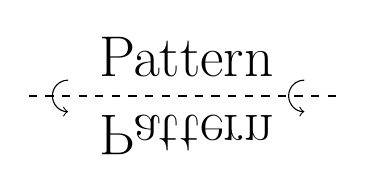
\begin{tikzpicture}
        % Draw the dashed line
        \draw[thick,dashed] (-2,0) -- (2,0);
        % Draw arcs
        \draw[->] (-1.5,0.2) arc (90:270:0.2);
        \draw[->] (1.5,0.2) arc (90:270:0.2);
        % Normal text above the line
        \node at (0,0.5) {\huge Pattern};
        % Mirrored text below the line
            \node[rotate=180] at (0,-0.5) {\reflectbox{\huge Pattern}};
    \end{tikzpicture}
    \caption{Reflections}
    \label{Reflection}
\end{subfigure}
\hfill
\begin{subfigure}{0.45\linewidth}
    \centering
    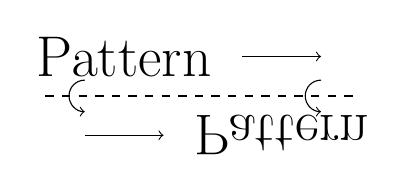
\begin{tikzpicture}
        % Draw the dashed line
        \draw[thick,dashed] (-2,0) -- (2,0);
        % Draw arcs
        \draw[->] (-1.5,0.2) arc (90:270:0.2);
        \draw[->] (1.5,0.2) arc (90:270:0.2);
        % Draw glide
        \draw[->] (0.5,0.5) -- (1.5,0.5);
        \draw[->] (-1.5,-0.5) -- (-0.5,-0.5);
        % Normal text above the line
        \node at (-1,0.5) {\huge Pattern};
        % Mirrored text below the line
            \node[rotate=180] at (1,-0.5) {\reflectbox{\huge Pattern}};
    \end{tikzpicture}
    \caption{Glide Reflection}
    \label{GlideReflection}
\end{subfigure}

\end{document}
        \caption{Reflective Symmetries}
        \label{fig:symmetries}
    \end{figure}
\end{frame}

\begin{frame}{Rotations}
    % \begin{definition}
        % A rotation is a change of angle around a center point.
        % $R_\theta = \begin{bmatrix}
        %     \cos\theta & -\sin\theta\\
        %     \sin\theta & \cos\theta
        % \end{bmatrix}$ 
        % Where $\theta \in \{1,2,3,6\}.$ \cite{Angela:2023}
    % \end{definition}
    \begin{figure}
        \centering
        \documentclass[class=article, crop=false]{standalone}
\usepackage{tikz}
\usepackage{subcaption}
\usetikzlibrary{calc}

\begin{document}

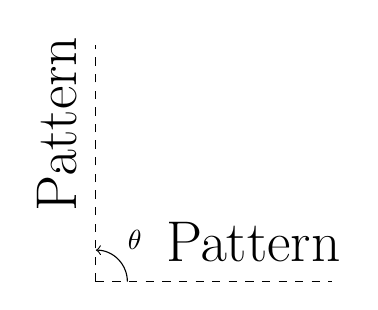
\begin{tikzpicture}
    \node[rotate=0] at ($(0:1) + (1,0.5)$) {\huge Pattern};
    \node[rotate=90] at ($(90:1) +(-0.5,1)$) {\huge Pattern};
    % Axis of rotation
    \draw[dashed] (0,0) -- (3,0);
    \draw[dashed] (0,0) -- (0,3);

    \draw[->] (0.4,0) arc (0:90:0.4) node[midway, above right] {$\theta$};
    %\node[] at (0,0) {o}
\end{tikzpicture}

\end{document}
        \caption{Rotations}
        \label{fig:enter-label}
    \end{figure}
\end{frame}

\begin{frame}{Frize Groups}
    \begin{figure}
        \centering
        % \documentclass[class=article, crop=false]{standalone}
\usepackage{tikz}
\usepackage{subcaption}
\usetikzlibrary{calc}

\begin{document}

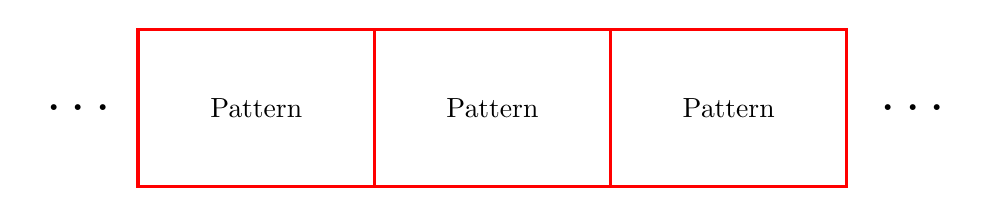
\begin{tikzpicture}
    \node[scale=2] at (-0.2, 1) {\ldots};
    \foreach \j in {0,...,2} {
        \draw[red, very thick] (0.5+3*\j,0) rectangle (3.5+3*\j,2);
        \node at (2 + 3*\j, 1) {Pattern};
    }
    % Add ellipsis at the end
    \node[scale=2] at (10.4, 1) {\ldots};
\end{tikzpicture}

\end{document}
        \input{diagrams/frieze-groups}
        \caption{Freize groups}
        \label{fig:Freize}
    \end{figure}
\end{frame}

\begin{frame}{Lattices}
    % \begin{definition}
        A lattice is the group $(\mathbb{Z}[\Vec{a},\Vec{b}],+).$\\
        i.e., a grid of points where any point $p = n\Vec{a} +m\Vec{b}$ 
    % \end{definition}
    \begin{figure}
        \centering
        \scalebox{0.5}{\documentclass[class=beamer, crop=false]{standalone}
\usepackage{tikz}
\usepackage{subcaption}
\usetikzlibrary{calc}

\begin{document}
\begin{tikzpicture}
            \def\a{2}  % length of side a
            \def\b{3}  % length of side b

            \foreach \i in {0,...,6} {
                \foreach \j in {0,...,3} {
                     \fill[blue]  (\i*\a,\j*\b) circle(3.5pt);
                }
            }
            % Draw vector
            \coordinate (P) at (3*\a, 2*\b);
            \draw[thick,->] (0,0) -- (P) node[above right] {\huge $p$};

            % Draw lattice parameters
            \draw (0,0) -- (\a,0) node[midway,below] {\huge$\Vec{b}$};
            \draw (0,0) -- (0,\b) node[midway,left] {\huge$\Vec{a}$};
        \end{tikzpicture}
\end{document}}
        \caption{Lattice}
        \label{fig:enter-label}
    \end{figure}
\end{frame}

\begin{frame}{Bravais lattices}
    \begin{enumerate}
        \item[(a)] Square:\hspace*{14pt} $||\vec{a}||=||\vec{b}|| < ||\vec{a}-\vec{b}|| = ||\vec{a}+\vec{b}||$

        \item[(b)] Hexagon:\hspace*{6pt} $||\vec{a}||=||\vec{b}|| = ||\vec{a}-\vec{b}|| < ||\vec{a}+\vec{b}||$

        \item[(c)] Rectangle: $||\vec{a}||<||\vec{b}|| < ||\vec{a}-\vec{b}|| = ||\vec{a}+\vec{b}||$

        \item[(d)] Rhombic:\hspace*{6pt} $||\vec{a}||<||\vec{b}|| = ||\vec{a}-\vec{b}|| < ||\vec{a}+\vec{b}||$

        \item[(e)] Oblique:\hspace*{11pt} $||\vec{a}||<||\vec{b}|| < ||\vec{a}-\vec{b}|| < ||\vec{a}+\vec{b}||$
    \end{enumerate}
\end{frame}

\begin{frame}{Bravais Lattices}
    \begin{figure}
        \centering
        % \resizebox{0.9\columnwidth}{!}{%
        \documentclass[class=beamer, crop=false]{standalone}

\usepackage{tikz}
\usepackage{subcaption}
\usetikzlibrary{calc}


\begin{document}

% \begin{figure}[0.8\linewidth]
  % \centering
  \begin{columns}[t]
      \centering
      \column{0.4\textwidth}
      \centering
    
      \resizebox{0.5\columnwidth}{!}{%
      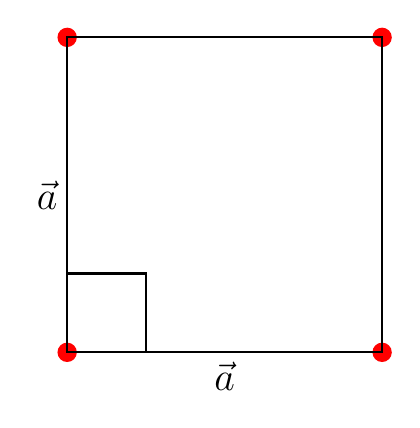
\begin{tikzpicture}
        \def\a{4}  % length of side a
            
        % Calculate the coordinates of the points
        \coordinate (A) at (0, 0);
        \coordinate (B) at (\a, 0);
        \coordinate (C) at (\a, \a);
        \coordinate (D) at (0, \a);
    
        \fill[red]  (A) circle(3.5pt) (B) circle(3.5pt) (C) circle(3.5pt) (D) circle(3.5pt);
            
        % Draw the square unit cell
        \draw[thick] (A) -- (B) -- (C) -- (D) -- cycle;
    
        % Draw right angle
        \draw[thick] (0,1) -- (1,1) -- (1,0);
    
        %Draw lattice parameters
        \node[left] at ($(A)!0.5!(D)$) {\Large $\vec{a}$};
        \node[below] at ($(A)!0.5!(B)$) {\Large $\vec{a}$};
        
      \end{tikzpicture}}
    
      
      \vspace{0.5ex}
    
      {\footnotesize\textbf{(a)} Square Cell}
    
      \column{0.4\textwidth}
        
      \resizebox{0.6\columnwidth}{!}{%
      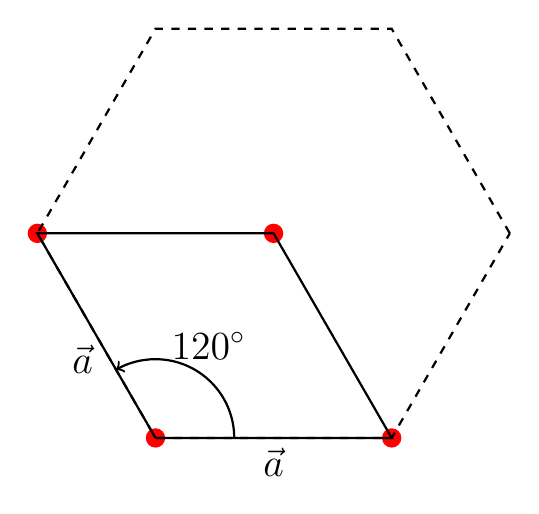
\begin{tikzpicture}
        \def\a{3}  % length of side a
            
        Calculate the coordinates of the points
        \coordinate (A) at (0:\a);
        \coordinate (B) at (60:\a);
        \coordinate (C) at (120:\a);
        \coordinate (D) at (180:\a);
        \coordinate (E) at (240:\a);
        \coordinate (F) at (300:\a);
        \coordinate (G) at (0,0);
       
        % Creates nodes at vertices
        \fill[red]  (D) circle(3.5pt) (E) circle(3.5pt) (F) circle(3.5pt) (G) circle(3.5pt);
        
        % Draw the hexagon boundary
        \draw[thick,dashed] (A) -- (B) -- (C) -- (D) -- (E) -- (F) -- (A);
    
        % Draw the cell
        \draw[thick] (E) -- (F) -- (G) -- (D) -- (E); 
            
        %Draw lattice parameters
        \node[anchor={60}] at ($(D)!0.5!(E)$) {\Large $\vec{a}$};
        \node[below] at ($(E)!0.5!(F)$) {\Large $\vec{a}$};
    
        % Optional: add angle markers
        \draw[thick, ->] (E) ++(1,0) arc[start angle=0, end angle=120, radius=1] node[midway,anchor={-120}] {\Large $120^\circ$};
        
      \end{tikzpicture}}
    
      {\footnotesize\textbf{(b)} Hexagon Cell}
    
    \end{columns}
    \vspace{1em}
    \begin{columns}[t]
      \centering
      \column{0.25\textwidth}
    
      \resizebox{0.9\columnwidth}{!}{%
      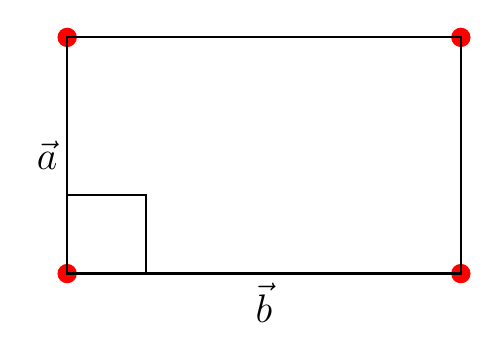
\begin{tikzpicture}
        \def\a{5}  % length of side a
        \def\b{3}  % length of side b
        \def\y{5}
    
        % Calculate the coordinates of the points
        \coordinate (A) at (0, 0);
        \coordinate (B) at (\a, 0);
        \coordinate (C) at (\a, \b);
        \coordinate (D) at (0, \b);
    
        % Creates nodes at vertices
        \fill[red]  (A) circle(3.5pt) (B) circle(3.5pt) (C) circle(3.5pt) (D) circle(3.5pt);
        
        % Draw right angle
        \draw[thick] (0,1) -- (1,1) -- (1,0);
    
        % Draw the rectangular unit cell
        \draw[thick] (A) -- (B) -- (C) -- (D) -- cycle;
       
        %Draw lattice parameters
        \node[left] at ($(A)!0.5!(D)$) {\Large $\vec{a}$};
        \node[below] at ($(A)!0.5!(B)$) {\Large $\vec{b}$};
    
      \end{tikzpicture}}
    
       \vspace{0.5ex}

       % Second row
    
      {\footnotesize\textbf{(c)} Rectangle Cell}
    
      \column{0.25\textwidth}
    
      \resizebox{0.9\columnwidth}{!}{%
      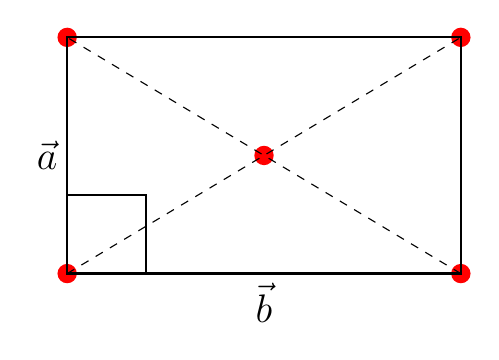
\begin{tikzpicture}
        \def\a{5}  % length of side a
        \def\b{3}  % length of side b
    
        % Calculate the coordinates of the points
        \coordinate (A) at (0, 0);
        \coordinate (B) at (\a, 0);
        \coordinate (C) at (\a, \b);
        \coordinate (D) at (0, \b);
    
        % Creates nodes at vertices
        \fill[red]  (A) circle(3.5pt) (B) circle(3.5pt) (C) circle(3.5pt) (D) circle(3.5pt);
        % Creates nodes at centers
        \fill[red] ($(A)!0.5!(C)$) circle(3.5pt);
    
        % Draw the rectangular unit cell
        \draw[thick] (A) -- (B) -- (C) -- (D) -- cycle;
    
        % Draw lines
        \draw[dashed] (A) -- (C);
        \draw[dashed] (B) -- (D);
    
        % Draw right angle
        \draw[thick] (0,1) -- (1,1) -- (1,0);
            
        %Draw lattice parameters
        \node[left] at ($(A)!0.5!(D)$) {\Large $\vec{a}$};
        \node[below] at ($(A)!0.5!(B)$) {\Large $\vec{b}$};
                
      \end{tikzpicture}}
    
      \vspace{0.5ex}
    
      {\footnotesize\textbf{(d)} Rhombic Cell}
    
      \column{0.3\textwidth}
    
      \resizebox{0.9\columnwidth}{!}{%
      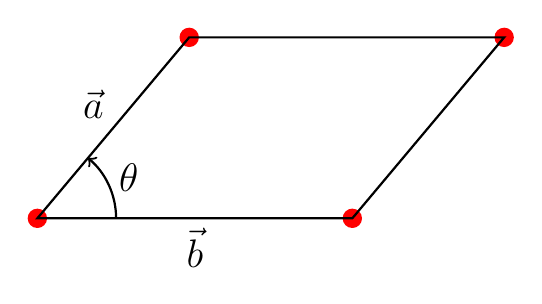
\begin{tikzpicture}
        % Define the lengths of the sides and the angle
        \def\a{4}  % length of side a
        \def\b{3}  % length of side b
        \def\angle{50}  % angle between sides a and b
    
        % Calculate the coordinates of the points
        \coordinate (A) at (0, 0);
        \coordinate (B) at (\a, 0);
        \coordinate (C) at ({\a + \b*cos(\angle)}, {\b * sin(\angle)});
        \coordinate (D) at ({\b * cos(\angle)}, {\b * sin(\angle)});
         
        % Creates nodes at vertices
        \fill[red]  (A) circle(3.5pt) (B) circle(3.5pt) (C) circle(3.5pt) (D) circle(3.5pt);
    
        % Draw the oblique unit cell
        \draw[thick] (A) -- (B) -- (C) -- (D) -- cycle;
    
        %Draw lattice parameters
        \node[anchor={-\angle}] at ($(A)!0.5!(D)$) {\Large $\vec{a}$};
        \node[below] at ($(A)!0.5!(B)$) {\Large $\vec{b}$};
        
        % Optional: add angle markers
        \draw[thick, ->] (A) ++(1,0) arc[start angle=0, end angle=\angle, radius=1] node[midway, anchor={150+\angle}] {\Large $\theta$};
      \end{tikzpicture}}
    
      \vspace{0.5ex}
    
      {\footnotesize\textbf{(e)} Oblique Cell}
    \end{columns}
  % \caption{All five two‐dimensional Bravais unit cells.}
  % \label{fig:bravais-cells}
% \end{figure}

\end{document}

        \caption{All five two‐dimensional Bravais lattice cells.}
        \label{fig:bravis-lattices}
    \end{figure}
    % \documentclass[class=beamer, crop=false]{standalone}

\usepackage{tikz}
\usepackage{subcaption}
\usetikzlibrary{calc}


\begin{document}

% \begin{figure}[0.8\linewidth]
  % \centering
  \begin{columns}[t]
      \centering
      \column{0.4\textwidth}
      \centering
    
      \resizebox{0.5\columnwidth}{!}{%
      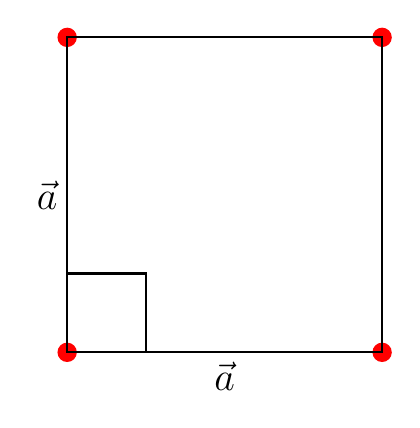
\begin{tikzpicture}
        \def\a{4}  % length of side a
            
        % Calculate the coordinates of the points
        \coordinate (A) at (0, 0);
        \coordinate (B) at (\a, 0);
        \coordinate (C) at (\a, \a);
        \coordinate (D) at (0, \a);
    
        \fill[red]  (A) circle(3.5pt) (B) circle(3.5pt) (C) circle(3.5pt) (D) circle(3.5pt);
            
        % Draw the square unit cell
        \draw[thick] (A) -- (B) -- (C) -- (D) -- cycle;
    
        % Draw right angle
        \draw[thick] (0,1) -- (1,1) -- (1,0);
    
        %Draw lattice parameters
        \node[left] at ($(A)!0.5!(D)$) {\Large $\vec{a}$};
        \node[below] at ($(A)!0.5!(B)$) {\Large $\vec{a}$};
        
      \end{tikzpicture}}
    
      
      \vspace{0.5ex}
    
      {\footnotesize\textbf{(a)} Square Cell}
    
      \column{0.4\textwidth}
        
      \resizebox{0.6\columnwidth}{!}{%
      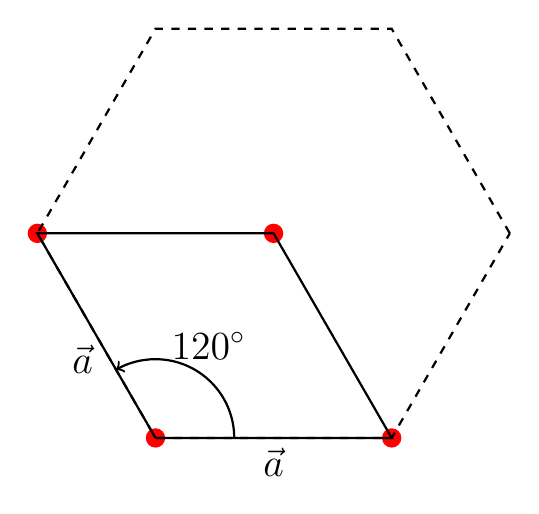
\begin{tikzpicture}
        \def\a{3}  % length of side a
            
        Calculate the coordinates of the points
        \coordinate (A) at (0:\a);
        \coordinate (B) at (60:\a);
        \coordinate (C) at (120:\a);
        \coordinate (D) at (180:\a);
        \coordinate (E) at (240:\a);
        \coordinate (F) at (300:\a);
        \coordinate (G) at (0,0);
       
        % Creates nodes at vertices
        \fill[red]  (D) circle(3.5pt) (E) circle(3.5pt) (F) circle(3.5pt) (G) circle(3.5pt);
        
        % Draw the hexagon boundary
        \draw[thick,dashed] (A) -- (B) -- (C) -- (D) -- (E) -- (F) -- (A);
    
        % Draw the cell
        \draw[thick] (E) -- (F) -- (G) -- (D) -- (E); 
            
        %Draw lattice parameters
        \node[anchor={60}] at ($(D)!0.5!(E)$) {\Large $\vec{a}$};
        \node[below] at ($(E)!0.5!(F)$) {\Large $\vec{a}$};
    
        % Optional: add angle markers
        \draw[thick, ->] (E) ++(1,0) arc[start angle=0, end angle=120, radius=1] node[midway,anchor={-120}] {\Large $120^\circ$};
        
      \end{tikzpicture}}
    
      {\footnotesize\textbf{(b)} Hexagon Cell}
    
    \end{columns}
    \vspace{1em}
    \begin{columns}[t]
      \centering
      \column{0.25\textwidth}
    
      \resizebox{0.9\columnwidth}{!}{%
      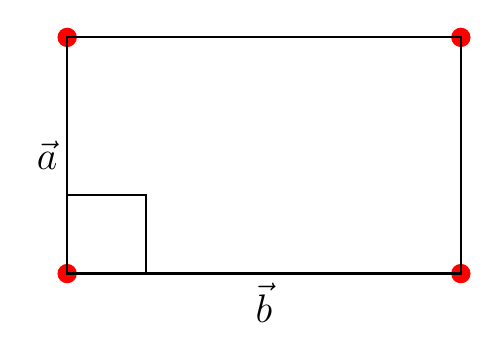
\begin{tikzpicture}
        \def\a{5}  % length of side a
        \def\b{3}  % length of side b
        \def\y{5}
    
        % Calculate the coordinates of the points
        \coordinate (A) at (0, 0);
        \coordinate (B) at (\a, 0);
        \coordinate (C) at (\a, \b);
        \coordinate (D) at (0, \b);
    
        % Creates nodes at vertices
        \fill[red]  (A) circle(3.5pt) (B) circle(3.5pt) (C) circle(3.5pt) (D) circle(3.5pt);
        
        % Draw right angle
        \draw[thick] (0,1) -- (1,1) -- (1,0);
    
        % Draw the rectangular unit cell
        \draw[thick] (A) -- (B) -- (C) -- (D) -- cycle;
       
        %Draw lattice parameters
        \node[left] at ($(A)!0.5!(D)$) {\Large $\vec{a}$};
        \node[below] at ($(A)!0.5!(B)$) {\Large $\vec{b}$};
    
      \end{tikzpicture}}
    
       \vspace{0.5ex}

       % Second row
    
      {\footnotesize\textbf{(c)} Rectangle Cell}
    
      \column{0.25\textwidth}
    
      \resizebox{0.9\columnwidth}{!}{%
      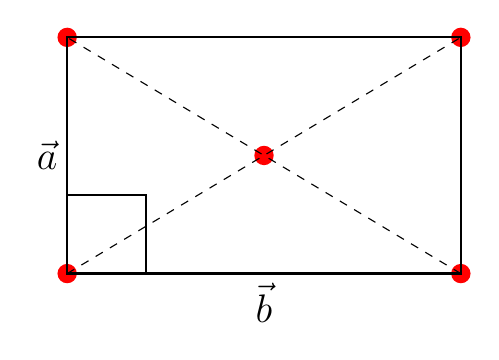
\begin{tikzpicture}
        \def\a{5}  % length of side a
        \def\b{3}  % length of side b
    
        % Calculate the coordinates of the points
        \coordinate (A) at (0, 0);
        \coordinate (B) at (\a, 0);
        \coordinate (C) at (\a, \b);
        \coordinate (D) at (0, \b);
    
        % Creates nodes at vertices
        \fill[red]  (A) circle(3.5pt) (B) circle(3.5pt) (C) circle(3.5pt) (D) circle(3.5pt);
        % Creates nodes at centers
        \fill[red] ($(A)!0.5!(C)$) circle(3.5pt);
    
        % Draw the rectangular unit cell
        \draw[thick] (A) -- (B) -- (C) -- (D) -- cycle;
    
        % Draw lines
        \draw[dashed] (A) -- (C);
        \draw[dashed] (B) -- (D);
    
        % Draw right angle
        \draw[thick] (0,1) -- (1,1) -- (1,0);
            
        %Draw lattice parameters
        \node[left] at ($(A)!0.5!(D)$) {\Large $\vec{a}$};
        \node[below] at ($(A)!0.5!(B)$) {\Large $\vec{b}$};
                
      \end{tikzpicture}}
    
      \vspace{0.5ex}
    
      {\footnotesize\textbf{(d)} Rhombic Cell}
    
      \column{0.3\textwidth}
    
      \resizebox{0.9\columnwidth}{!}{%
      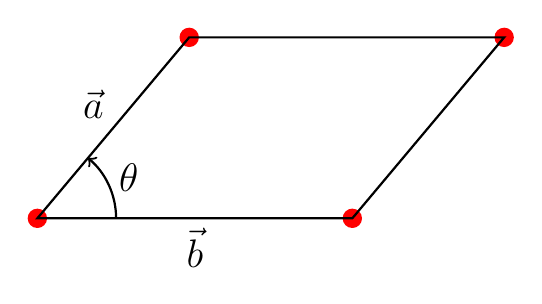
\begin{tikzpicture}
        % Define the lengths of the sides and the angle
        \def\a{4}  % length of side a
        \def\b{3}  % length of side b
        \def\angle{50}  % angle between sides a and b
    
        % Calculate the coordinates of the points
        \coordinate (A) at (0, 0);
        \coordinate (B) at (\a, 0);
        \coordinate (C) at ({\a + \b*cos(\angle)}, {\b * sin(\angle)});
        \coordinate (D) at ({\b * cos(\angle)}, {\b * sin(\angle)});
         
        % Creates nodes at vertices
        \fill[red]  (A) circle(3.5pt) (B) circle(3.5pt) (C) circle(3.5pt) (D) circle(3.5pt);
    
        % Draw the oblique unit cell
        \draw[thick] (A) -- (B) -- (C) -- (D) -- cycle;
    
        %Draw lattice parameters
        \node[anchor={-\angle}] at ($(A)!0.5!(D)$) {\Large $\vec{a}$};
        \node[below] at ($(A)!0.5!(B)$) {\Large $\vec{b}$};
        
        % Optional: add angle markers
        \draw[thick, ->] (A) ++(1,0) arc[start angle=0, end angle=\angle, radius=1] node[midway, anchor={150+\angle}] {\Large $\theta$};
      \end{tikzpicture}}
    
      \vspace{0.5ex}
    
      {\footnotesize\textbf{(e)} Oblique Cell}
    \end{columns}
  % \caption{All five two‐dimensional Bravais unit cells.}
  % \label{fig:bravais-cells}
% \end{figure}

\end{document}

\end{frame}



\begin{frame}{Wallpaper groups}
    \begin{figure}
        \centering
        % \input{diagrams/Wallpaper Group Diagrams/AllGroups}
        \documentclass[class=beamer, crop=false]{standalone}
%\documentclass[12pt]{article}
\usepackage{tikz}
\usepackage{subcaption}
\usetikzlibrary{calc}
\usetikzlibrary {shapes.geometric}
\usepackage{graphicx}
\usepackage{standalone} 


\begin{document}

% \begin{frame}{The 17 Wallpaper Groups}

  % ─── First row: 6 diagrams ───────────────────────────────────────────
  %── p1 ─────────────────────────────────────────────────────────────
  \begin{minipage}[t]{0.20\textwidth}
    \centering
    \includestandalone[width=\linewidth]{diagrams/wallpaper-groups/p1}\\[-0.5ex]
    {\footnotesize\textbf{p1}}
  \end{minipage}%
  \hspace{-0.4em}% ← adjust this
  %── p2 ─────────────────────────────────────────────────────────────
  \begin{minipage}[t]{0.17\textwidth}
    \centering
    \includestandalone[width=\linewidth]{diagrams/wallpaper-groups/p2}\\[-0.5ex]
    {\footnotesize\textbf{p2}}
  \end{minipage}%
  \hspace{0.2em}% ← adjust this
  %── pm ─────────────────────────────────────────────────────────────
  \begin{minipage}[t]{0.15\textwidth}
    \centering
    \includestandalone[width=\linewidth]{diagrams/wallpaper-groups/pm}\\[-0.5ex]
    {\footnotesize\textbf{pm}}
  \end{minipage}%
  \hspace{0.5em}% ← adjust this
  %── pg ─────────────────────────────────────────────────────────────
  \begin{minipage}[t]{0.14\textwidth}
    \centering
    \includestandalone[width=\linewidth]{diagrams/wallpaper-groups/pg}\\[-0.5ex]
    {\footnotesize\textbf{pg}}
  \end{minipage}%
  \hspace{0.2em}% ← adjust this
  %── cm ─────────────────────────────────────────────────────────────
  \begin{minipage}[t]{0.145\textwidth}
    \centering
    \includestandalone[width=\linewidth]{diagrams/wallpaper-groups/cm}\\[-0.5ex]
    {\footnotesize\textbf{cm}}
  \end{minipage}%
  \hspace{0.2em}% ← adjust this
  %── pmm ────────────────────────────────────────────────────────────
  \begin{minipage}[t]{0.15\textwidth}
    \centering
    \includestandalone[width=\linewidth]{diagrams/wallpaper-groups/pmm}\\[-0.5ex]
    {\footnotesize\textbf{pmm}}
  \end{minipage}

  \vspace{1em}

  % ─── Second row: 6 diagrams ──────────────────────────────────────────
  \begin{columns}[t,onlytextwidth]
    \column{0.15\textwidth}\centering
      \includestandalone[width=0.9\columnwidth]{diagrams/wallpaper-groups/pmg}
      \\[-0.5ex]\footnotesize\textbf{pmg}

    \column{0.15\textwidth}\centering
      \includestandalone[width=0.9\columnwidth]{diagrams/wallpaper-groups/pgg}
      \\[-0.5ex]\footnotesize\textbf{pgg}

    \column{0.16\textwidth}\centering
      \includestandalone[width=0.9\columnwidth]{diagrams/wallpaper-groups/cmm}
      \\[-0.5ex]\footnotesize\textbf{cmm}

      \column{0.16\textwidth}\centering
      \includestandalone[width=0.9\columnwidth]{diagrams/wallpaper-groups/p4}
      \\[-0.5ex]\footnotesize\textbf{p4}

    \column{0.16\textwidth}\centering
      \includestandalone[width=0.9\columnwidth]{diagrams/wallpaper-groups/p4m}
      \\[-0.5ex]\footnotesize\textbf{p4m}

    \column{0.16\textwidth}\centering
      \includestandalone[width=0.9\columnwidth]{diagrams/wallpaper-groups/p4g}
      \\[-0.5ex]\footnotesize\textbf{p4g}

  \end{columns}

  \vspace{1em}

  % ─── Third row: 5 diagrams ───────────────────────────────────────────
  \begin{minipage}[t]{0.2\textwidth}
    \centering
    \includestandalone[width=\linewidth]{diagrams/wallpaper-groups/p3}\\[-0.5ex]
    {\footnotesize\textbf{p3}}
  \end{minipage}%
  % \hspace{-0.2em}% <<–– try -0.8em, -1em, -1.2em etc.
  \begin{minipage}[t]{0.19\textwidth}
    \centering
    \includestandalone[width=\linewidth]{diagrams/wallpaper-groups/p3m1}\\[-0.5ex]
    {\footnotesize\textbf{p3m1}}
  \end{minipage}%
  % \hspace{-0.2em}%
  \begin{minipage}[t]{0.2\textwidth}
    \centering
    \includestandalone[width=\linewidth]{diagrams/wallpaper-groups/p31m}\\[-0.5ex]
    {\footnotesize\textbf{p31m}}
  \end{minipage}%
  % \hspace{-0.2em}%
  \begin{minipage}[t]{0.2\textwidth}
    \centering
    \includestandalone[width=\linewidth]{diagrams/wallpaper-groups/p6}\\[-0.5ex]
    {\footnotesize\textbf{p6}}
  \end{minipage}%
  % \hspace{-0.2em}%
  \begin{minipage}[t]{0.2\textwidth}
    \centering
    \includestandalone[width=\linewidth]{diagrams/wallpaper-groups/p6m}\\[-0.5ex]
    {\footnotesize\textbf{p6m}}
  \end{minipage}

% \end{frame}

\end{document}

        \caption{The 17 wallpaper groups }
        \label{fig:17WallpaperGroups}
    \end{figure}
\end{frame}

\begin{frame}{Classification of wallpaper groups}
    p and c refer to primitive centred cells, respectively.

\end{frame}

\begin{frame}{Oblique patterns}
  \begin{figure}
    \centering
    % left box, top-aligned
    \begin{minipage}[t]{0.50\textwidth}
      \centering
      \includestandalone[width=\linewidth]{diagrams/wallpaper-groups/p1}
      \caption*{\texttt{p1}}
    \end{minipage}\hspace{0cm}%
    % right box, top-aligned
    \begin{minipage}[t]{0.45\textwidth}
      \centering
      \includestandalone[width=\linewidth]{diagrams/wallpaper-groups/p2}
      \caption*{\texttt{p2}}
    \end{minipage}
    \caption{lattice diagrams for oblique cells}
  \end{figure}
\end{frame}

\begin{frame}{Square patterns}
  \begin{figure}
    \centering
    % left box, top-aligned
    \begin{minipage}[t]{0.32\textwidth}
      \centering
      \includestandalone[width=\linewidth]{diagrams/wallpaper-groups/p4}
      \caption*{\texttt{p4}}
    \end{minipage}\hfill%
    % middle box, top-aligned
    \begin{minipage}[t]{0.32\textwidth}
      \centering
      \includestandalone[width=\linewidth]{diagrams/wallpaper-groups/p4m}
      \caption*{\texttt{p4m}}
    \end{minipage}\hfill
    % right box, top-aligned
    \begin{minipage}[t]{0.32\textwidth}
      \centering
      \includestandalone[width=\linewidth]{diagrams/wallpaper-groups/p4g}
      \caption*{\texttt{p4g}}
    \end{minipage}
    \caption{lattice diagrams for square cells}
  \end{figure}
\end{frame}

\begin{frame}{Rectangle patterns}
  \begin{figure}
    \centering
    % ——— Top row: 3 cells ———
    \begin{minipage}[t]{0.31\textwidth}
      \centering
      \includestandalone[width=\linewidth]{diagrams/wallpaper-groups/pm}
      \caption*{\texttt{pm}}
    \end{minipage}\hspace{1.cm5}
    \begin{minipage}[t]{0.28\textwidth}
      \centering
      \includestandalone[width=\linewidth]{diagrams/wallpaper-groups/pg}
      \caption*{\texttt{pg}}
    \end{minipage}
    
    % \vspace{1em} % space between rows

    % ——— Bottom row: 2 cells ———
    \begin{minipage}[t]{0.29\textwidth}
      \centering
      \includestandalone[width=\linewidth]{diagrams/wallpaper-groups/pmm}
      \caption*{\texttt{pmm}}
    \end{minipage}\hfill
    \begin{minipage}[t]{0.3\textwidth}
      \centering
      \includestandalone[width=\linewidth]{diagrams/wallpaper-groups/pmg}
      \caption*{\texttt{pmg}}
    \end{minipage}\hfill
    \begin{minipage}[t]{0.3\textwidth}
      \centering
      \includestandalone[width=\linewidth]{diagrams/wallpaper-groups/pgg}
      \caption*{\texttt{pgg}}
    \end{minipage}

    \caption{Lattice diagrams for rectangle cells (\texttt{pm}, \texttt{pg}, \texttt{pmm}, \texttt{pmg}, \texttt{pgg}).}
  \end{figure}
\end{frame}



\begin{frame}{Rhombic patterns}
  \begin{figure}
    \centering
    % left box, top-aligned
    \begin{minipage}[t]{0.45\textwidth}
      \centering
      \includestandalone[width=\linewidth]{diagrams/wallpaper-groups/cm}
      \caption*{\texttt{cm}}
    \end{minipage}\hfill%
    % right box, top-aligned
    \begin{minipage}[t]{0.45\textwidth}
      \centering
      \includestandalone[width=\linewidth]{diagrams/wallpaper-groups/cmm}
      \caption*{\texttt{cmm}}
    \end{minipage}
    \caption{lattice diagrams for rhombic cells}
  \end{figure}
\end{frame}

\begin{frame}{Hexagon patterns}
  \begin{figure}
    \centering
    % ——— Top row: 3 cells ———
    \begin{minipage}[t]{0.31\textwidth}
      \centering
      \includestandalone[width=\linewidth]{diagrams/wallpaper-groups/p3}
      \caption*{\texttt{p3}}
    \end{minipage}\hspace{-0.5cm}
    \begin{minipage}[t]{0.31\textwidth}
      \centering
      \includestandalone[width=\linewidth]{diagrams/wallpaper-groups/p31m}
      \caption*{\texttt{p31m}}
    \end{minipage}\hspace{-0.5cm}
    \begin{minipage}[t]{0.31\textwidth}
      \centering
      \includestandalone[width=\linewidth]{diagrams/wallpaper-groups/p31m}
      \caption*{\texttt{p31m}}
    \end{minipage}

    % \vspace{1em} % space between rows

    % ——— Bottom row: 2 cells ———
    \begin{minipage}[t]{0.32\textwidth}
      \centering
      \includestandalone[width=\linewidth]{diagrams/wallpaper-groups/p6}
      \caption*{\texttt{p6}}
    \end{minipage}
    \begin{minipage}[t]{0.32\textwidth}
      \centering
      \includestandalone[width=\linewidth]{diagrams/wallpaper-groups/p6m}
      \caption*{\texttt{p6m}}
    \end{minipage}

    \caption{Lattice diagrams for hexagon cells (\texttt{pm}, \texttt{pg}, \texttt{pmm}, \texttt{pmg}, \texttt{pgg}).}
  \end{figure}
\end{frame}

\begin{frame}{Subgroups}
  \begin{table}
    \centering
    \begin{tabular}{@{} ll @{\qquad} ll @{}}
      \toprule
      \textbf{G} & \textbf{H} & \textbf{G} & \textbf{H} \\
      \midrule
      p1   & trivial                          & p4    & $\mathbb{Z}_4$              \\
      p2   & $\mathbb{Z}_2$                   & p4m   & $D_4$                       \\
      pm   & $\mathbb{Z}_2$                   & p4g   & $D_4$                       \\
      pg   & $\mathbb{Z}_2$                   & p3    & $\mathbb{Z}_3$              \\
      pmm  & $\mathbb{Z}_2\times\mathbb{Z}_2$ & p3m1  & $D_3$                       \\
      pmg  & $\mathbb{Z}_2\times\mathbb{Z}_2$ & p31m  & $D_3$                       \\
      pgg  & $\mathbb{Z}_2\times\mathbb{Z}_2$ & p6    & $\mathbb{Z}_6$              \\
      cm   & $\mathbb{Z}_2$                   & p6m   & $D_6$                       \\
      cmm  & $\mathbb{Z}_2\times\mathbb{Z}_2$ &       &                             \\
      \bottomrule
    \end{tabular}
    \caption{Wallpaper groups \(G\) and their corresponding symmetry subgroups \(H\).} \cite{sasse_2020}
  \end{table}
\end{frame}


\begin{frame}{Hilbert problems}
    
\end{frame}

\begin{frame}{Penrose Tilling}
    \begin{figure}
        \centering
        \includegraphics[width=0.5\linewidth]{images/Penrose_Tiling_(Rhombi).svg.png}
        \caption{Penrose tilling}
        \label{fig:penrose-rhombi}
    \end{figure}
\end{frame}

\begin{frame}{The Einstein("One Tile") problem}
    Is it possible to tile a plane using a single tile that only tiles aperiodically.
\end{frame}

\begin{frame}{The Hat}
    In 2023 Smith,Myers,Kaplan and Goodman-Strauss proved that the the hat
\end{frame}

\begin{frame}{Proof sketch}
    
\end{frame}

\begin{frame}{Metatiles}
    \begin{figure}
        \centering
        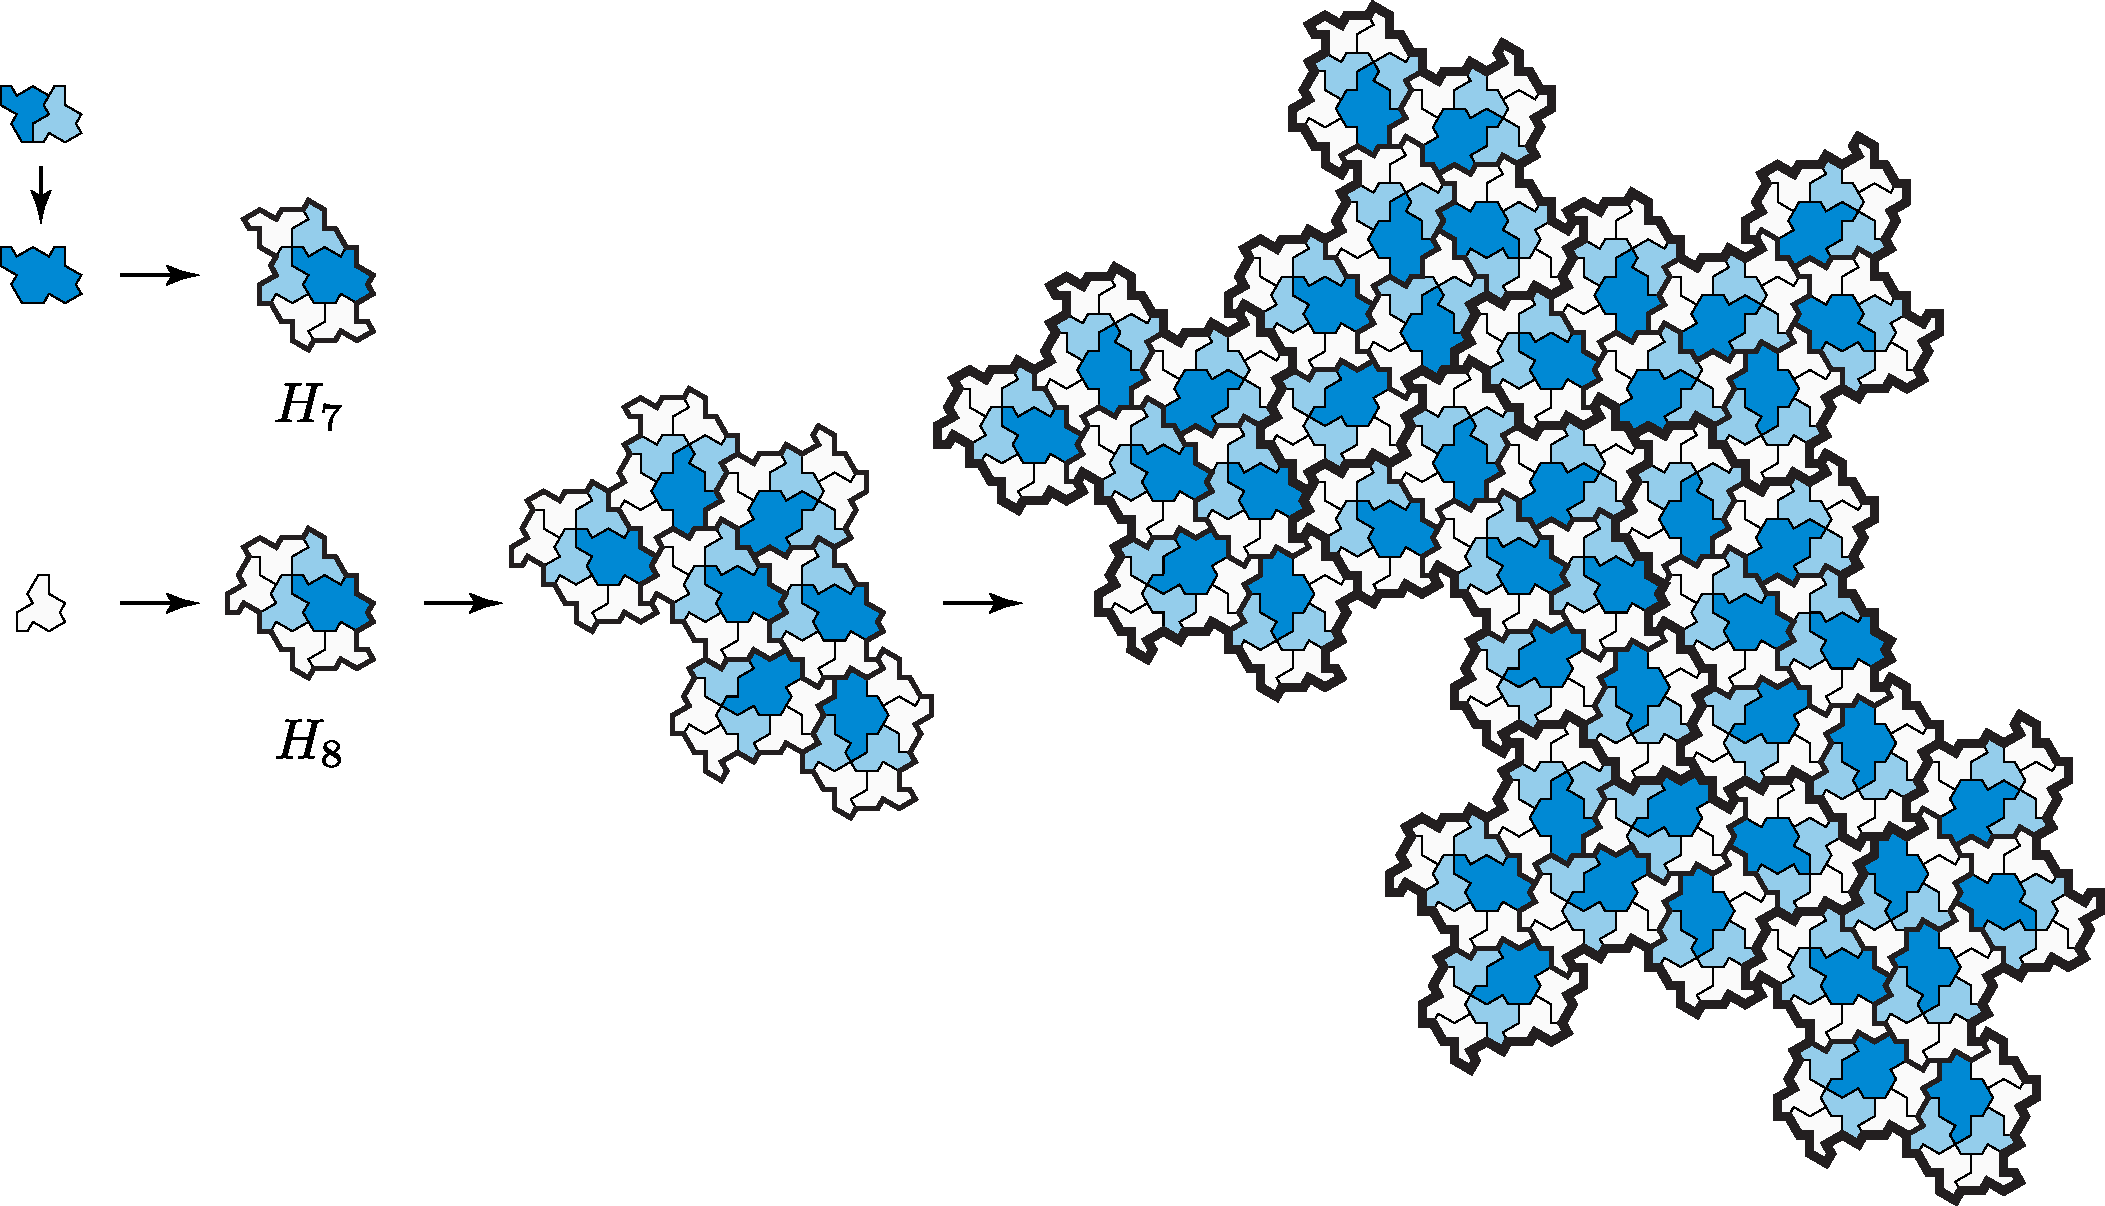
\includegraphics[page=1,width=\textwidth]{images/aperiodic-pdfs/alt_subst.pdf}
        \caption{A metatile of the hat}
        \label{fig:hat-metatile}
    \end{figure}
\end{frame}

% \begin{frame}{Other polykites}
%     \begin{figure}
%         \centering
%         \begin{minipage}[width=0.24\textwidth]
%             \centering
%             \includegraphics[\linewidth]{images/polykite-family/chevron(0,1).png}
%         \end{minipage} \hfill
%         \begin{minipage}[width=0.24\textwidth]
%             \centering
%             \includegraphics[\linewidth]{images/polykite-family/tile(1,4).png}
%         \end{minipage} \hfill
%         \begin{minipage}[width=0.24\linewidth]
%             \centering
%             \includegraphics[\linewidth]{images/polykite-family/hat(1,sqrt(3)).png}
%         \end{minipage} \hfill
%         \begin{minipage}[width=0.24\textwidth]
%             \centering
%             \includegraphics[\linewidth]{images/polykite-family/tile(1,1).png}
%         \end{minipage}
%         \caption{Caption}
%         \label{fig:enter-label}
%     \end{figure}
% \end{frame}

\begin{frame}{The Spectre}
    Shortly after their groundbreaking paper they were able to add a chirality to the tile and aperiodically tile the plane without mirrors.
    \begin{figure}
        \centering
        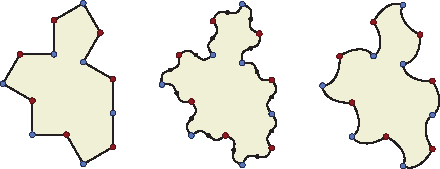
\includegraphics[width=\linewidth]{images/aperiodic-pdfs/polygon_to_spectre.pdf}
        \caption{From the turtle to the spectre}
        \label{fig:turle-spectra}
    \end{figure}
\end{frame}

\begin{frame}{Family of polykites}
    \begin{figure}
        \centering
        \includegraphics[width=\textwidth]{images/polykite-family/monotile-continuum.png}
        \caption{Family of poly-kites and the spectre}
        \label{fig:poly-kites-spectre}
    \end{figure}
\end{frame}

% \begin{frame}{The Spectre}
%     \includesvg[width=0.8\textwidth]{images/Spectre_aperiodic_monotile_single.svg}
% \end{frame}

\begin{frame}{GitHub}
    \begin{figure}
        \centering
        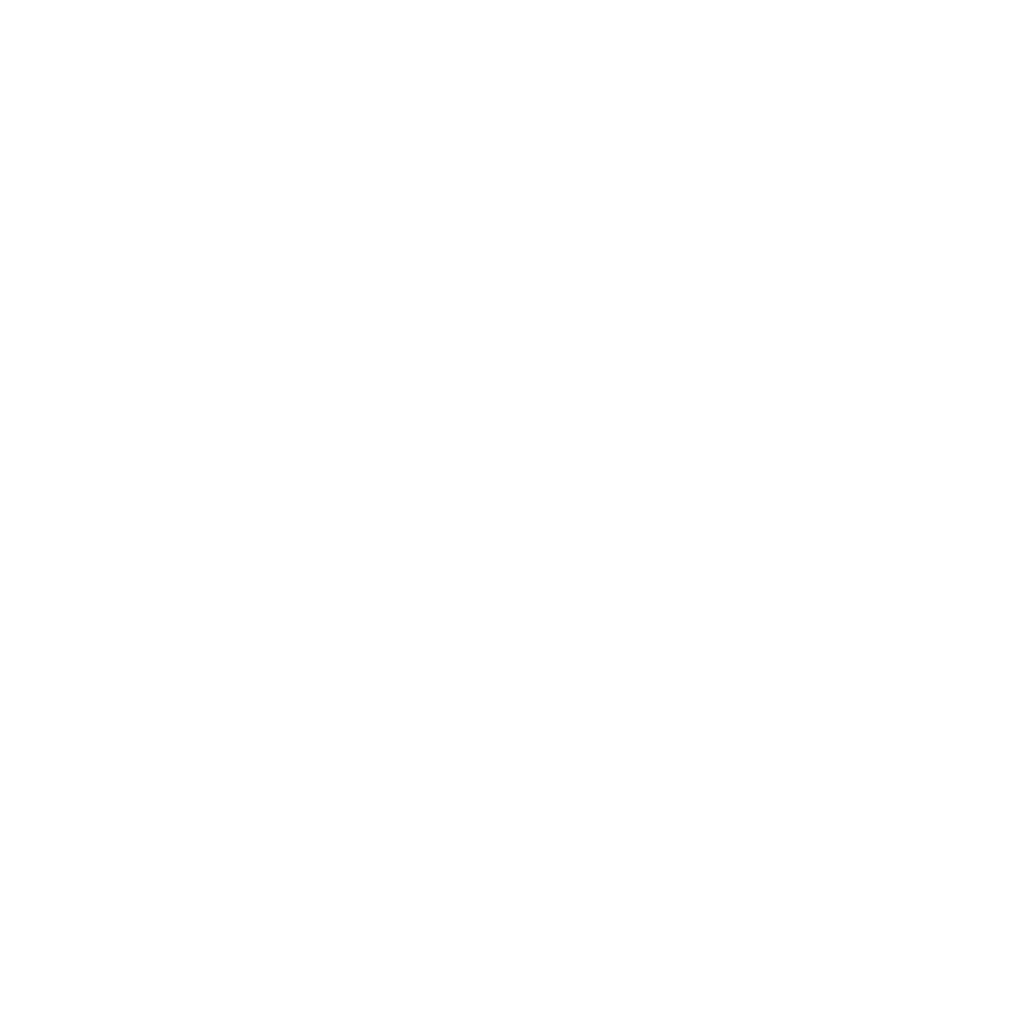
\includegraphics[width=0.6\textwidth]{images/qr-codes/tilling-presentation-github.png}
        \caption{GitHub}
        \label{fig:github-qrcode}
    \end{figure}
\end{frame}

\begin{frame}{resourses}
    \begin{itemize}
        \item \href{https://www.youtube.com/watch?v=_ZS3Oqg1AX0&ab_channel=Numberphile}{Numberphile interview with Graig Kaplan}
        \item \href{https://ms.unimelb.edu.au/__data/assets/pdf_file/0011/5218382/vujamie_296128_22162633_Jamie_Vu_Poster_final.pdf}{Posture from Melbourne student}
        \item href{https://cs.uwaterloo.ca/~csk/spectre/app.html}{Interactive web}
    \end{itemize}
\end{frame}

\begin{frame}{References}
    
\end{frame}


%% Axuillary slides

\begin{frame}{Appendices}
    Other information
\end{frame}

% \begin{frame}{P1 Wallpaper Group}
    \begin{figure}
        \centering
        \documentclass[class=article, crop=false]{standalone}
\usepackage{tikz}
\usepackage{subcaption}
\usetikzlibrary{calc}

\begin{document}
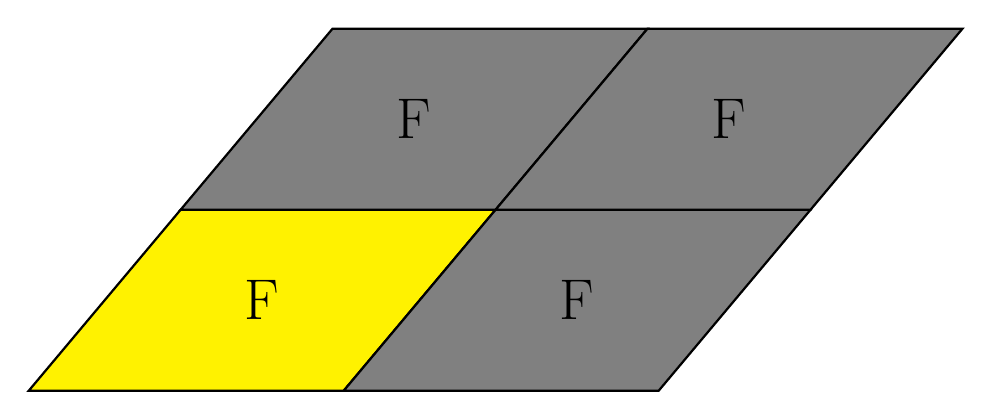
\begin{tikzpicture}
    % Define the lengths of the sides and the angle
    \def\a{4}  % length of side a
    \def\b{3}  % length of side b
    \def\angle{50}  % angle between sides a and b
    \def\s{F} % Label in center of cells

    % Calculate the coordinates of the points
    \coordinate (C00) at (0, 0);
    \coordinate (C10) at (\a, 0);
    \coordinate (C11) at ({\a + \b*cos(\angle)}, {\b * sin(\angle)});
    \coordinate (C01) at ({\b * cos(\angle)}, {\b * sin(\angle)});
    \coordinate (C02) at ({2*\b*cos(\angle)}, {2*\b * sin(\angle)});
    \coordinate (C12) at ({\a +2*\b * cos(\angle)}, {2*\b * sin(\angle)});
    \coordinate (C22) at ({2*\a + 2*\b * cos(\angle)}, {2*\b * sin(\angle)});
    \coordinate (C21) at ({2*\a + \b*cos(\angle)}, {\b * sin(\angle)});
    \coordinate (C20) at ({2*\a}, 0);

        
    % Draw the oblique unit cell
    \draw[thick,fill=yellow] (C00) -- (C10) -- (C11) -- (C01) -- cycle;
    \draw[thick,fill=gray] (C01) -- (C11) -- (C12) -- (C02) -- cycle;
    \draw[thick,fill=gray] (C10) -- (C20) -- (C21) -- (C11) -- cycle;
    \draw[thick,fill=gray] (C11) -- (C21) -- (C22) -- (C12) -- cycle;

    % Center symbols
    \node at ($(C00)!0.5!(C11)$) {\huge \s};
    \node at ($(C20)!0.5!(C11)$) {\huge \s};
    \node at ($(C02)!0.5!(C11)$) {\huge \s};
    \node at ($(C22)!0.5!(C11)$) {\huge \s};
\end{tikzpicture}
\end{document}
        \caption{p1}
        \label{fig:p1}
    \end{figure}
\end{frame}

\begin{frame}{P2 Wallpaper Group}
    \begin{figure}
        \centering
        \documentclass[class=article, crop=false]{standalone}
\usepackage{tikz}
\usepackage{subcaption}
\usetikzlibrary{calc}
\usetikzlibrary {shapes.geometric}

\begin{document}
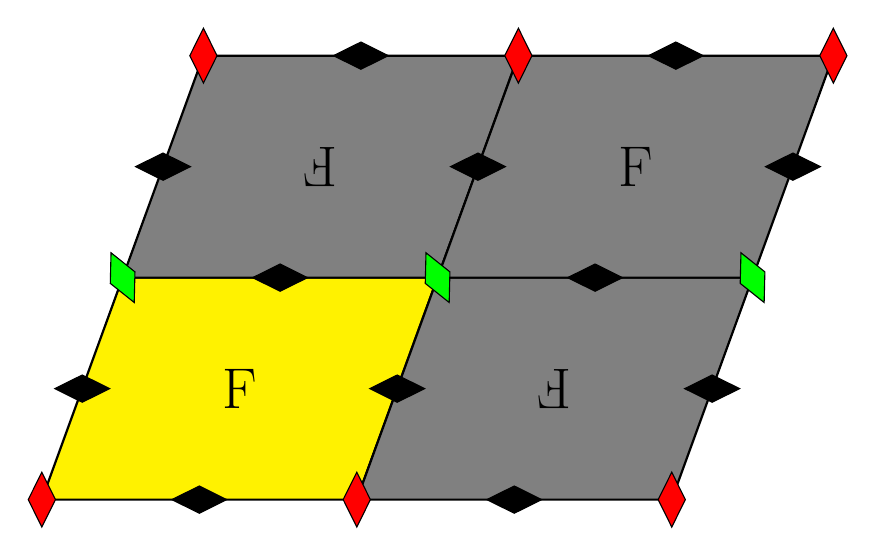
\begin{tikzpicture}
    % Define the lengths of the sides and the angle
    \def\a{4}  % length of side a
    \def\b{3}  % length of side b
    \def\angle{70}  % angle between sides a and b
    \def\s{F} % Label in center of cells

    % Calculate the coordinates of the points
    \coordinate (C00) at (0, 0);
    \coordinate (C10) at (\a, 0);
    \coordinate (C11) at ({\a + \b*cos(\angle)}, {\b * sin(\angle)});
    \coordinate (C01) at ({\b * cos(\angle)}, {\b * sin(\angle)});
    \coordinate (C02) at ({2*\b*cos(\angle)}, {2*\b * sin(\angle)});
    \coordinate (C12) at ({\a +2*\b * cos(\angle)}, {2*\b * sin(\angle)});
    \coordinate (C22) at ({2*\a + 2*\b * cos(\angle)}, {2*\b * sin(\angle)});
    \coordinate (C21) at ({2*\a + \b*cos(\angle)}, {\b * sin(\angle)});
    \coordinate (C20) at ({2*\a}, 0);
        
    % Draw the oblique unit cell
    \draw[thick,fill=yellow] (C00) -- (C10) -- (C11) -- (C01) -- cycle;
    \draw[thick,fill=gray] (C10) -- (C20) -- (C21) -- (C11) -- cycle;
    \draw[thick,fill=gray] (C01) -- (C11) -- (C12) -- (C02) -- cycle;
    \draw[thick,fill=gray] (C11) -- (C21) -- (C22) -- (C12) -- cycle;
    
    % Draw chiral center
    \node at ($(C00)!0.5!(C11)$) {\huge \s};
    \node[rotate=180] at ($(C01)!0.5!(C12)$) {\huge \s};
    \node at ($(C11)!0.5!(C22)$) {\huge \s};
    \node[rotate=180] at ($(C10)!0.5!(C21)$) {\huge \s};

    % Draw node reflections
    \draw (C00)  node[shape aspect=0.5,diamond,draw,fill=red] {};
    \draw (C10)  node[shape aspect=0.5,diamond,draw,fill=red] {};
    \draw (C20)  node[shape aspect=0.5,diamond,draw,fill=red] {};
    \draw (C01)  node[rotate = \angle-45,shape aspect=0.5,diamond,draw,fill=green] {};
    \draw (C11)  node[rotate = \angle-45,shape aspect=0.5,diamond,draw,fill=green] {};
    \draw (C21)  node[rotate = \angle-45,shape aspect=0.5,diamond,draw,fill=green] {};
    \draw (C02)  node[shape aspect=0.5,diamond,draw,fill=red] {};
    \draw (C12)  node[shape aspect=0.5,diamond,draw,fill=red] {};
    \draw (C22)  node[shape aspect=0.5,diamond,draw,fill=red] {}; 
    \draw ($(C00)!0.5!(C10)$)  node[rotate=90,shape aspect=0.5,diamond,draw,fill=black] {};
    \draw ($(C10)!0.5!(C20)$)  node[rotate=90,shape aspect=0.5,diamond,draw,fill=black] {};
    \draw ($(C00)!0.5!(C01)$)  node[rotate=90,shape aspect=0.5,diamond,draw,fill=black] {};
    \draw ($(C10)!0.5!(C11)$)  node[rotate=90,shape aspect=0.5,diamond,draw,fill=black] {};
    \draw ($(C20)!0.5!(C21)$)  node[rotate=90,shape aspect=0.5,diamond,draw,fill=black] {};
    \draw ($(C01)!0.5!(C02)$)  node[rotate=90,shape aspect=0.5,diamond,draw,fill=black] {};
    
    \draw ($(C01)!0.5!(C11)$)  node[rotate=90,shape aspect=0.5,diamond,draw,fill=black] {};
    \draw ($(C11)!0.5!(C21)$)  node[rotate=90,shape aspect=0.5,diamond,draw,fill=black] {};
    
    \draw ($(C11)!0.5!(C12)$)  node[rotate=90,shape aspect=0.5,diamond,draw,fill=black] {};
    \draw ($(C21)!0.5!(C22)$)  node[rotate=90,shape aspect=0.5,diamond,draw,fill=black] {};
    \draw ($(C02)!0.5!(C12)$)  node[rotate=90,shape aspect=0.5,diamond,draw,fill=black] {};
    \draw ($(C12)!0.5!(C22)$)  node[rotate=90,shape aspect=0.5,diamond,draw,fill=black] {};
\end{tikzpicture}
\end{document}
        \caption{p2}
        \label{fig:p2}
    \end{figure}
\end{frame}

\begin{frame}{P4 Wallpaper Group}
    \begin{figure}
        \centering
        \input{diagrams/wallpaper-groups/p4}
        \caption{p4}
        \label{fig:p4}
    \end{figure}
\end{frame}

\begin{frame}{P4M Wallpaper Group}
    \begin{figure}
        \centering
        \documentclass[class=article, crop=false]{standalone}
\usepackage{tikz}
\usepackage{subcaption}
\usetikzlibrary{calc}
\usetikzlibrary {shapes.geometric}

\begin{document}
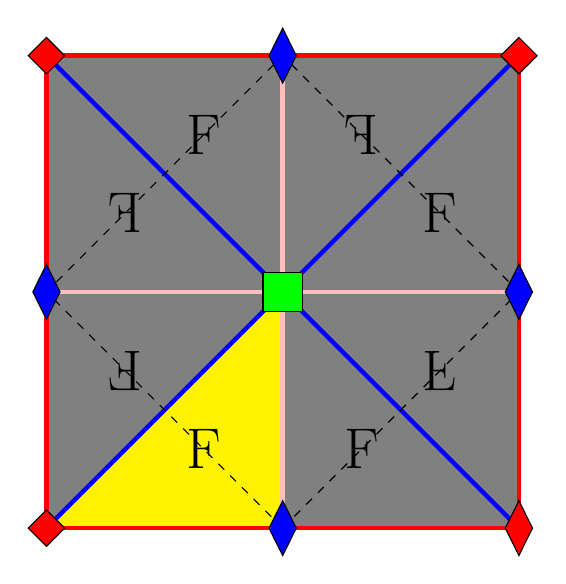
\begin{tikzpicture}
            % Define the lengths of the sides and the angle
            \def\a{3}  % length of side a
            \def\b{3}  % length of side b
            \def\angle{90}  % angle between sides a and b
            \def\s{F}
        
            % Calculate the coordinates of the points
            \coordinate (C00) at (0, 0);
            \coordinate (C10) at (\a, 0);
            \coordinate (C11) at ({\a + \b*cos(\angle)}, {\b * sin(\angle)});
            \coordinate (C01) at ({\b * cos(\angle)}, {\b * sin(\angle)});
            \coordinate (C02) at ({2*\b*cos(\angle)}, {2*\b * sin(\angle)});
            \coordinate (C12) at ({\a +2*\b * cos(\angle)}, {2*\b * sin(\angle)});
            \coordinate (C22) at ({2*\a + 2*\b * cos(\angle)}, {2*\b * sin(\angle)});
            \coordinate (C21) at ({2*\a + \b*cos(\angle)}, {\b * sin(\angle)});
            \coordinate (C20) at ({2*\a}, 0);
        
            % Draw the oblique unit cell
            \draw[thick,fill=gray] (C00) -- (C20) -- (C22) -- (C02) -- cycle;
            \draw[thick,fill=yellow] (C00) -- (C10) -- (C11) -- cycle;
            \draw[ultra thick,red] (C00) -- (C20) -- (C22) -- (C02) -- cycle;
            \draw[ultra thick,blue] (C11) -- (C00);
            \draw[ultra thick,blue] (C11) -- (C20);
            \draw[ultra thick,blue] (C11) -- (C22);
            \draw[ultra thick,blue] (C11) -- (C02);
            \draw[ultra thick,pink] (C11) -- (C10);
            \draw[ultra thick,pink] (C11) -- (C21);
            \draw[ultra thick,pink] (C11) -- (C12);
            \draw[ultra thick,pink] (C11) -- (C01);
            
            % Draw mirrow lines
            \draw[dashed] (C10) -- (C21) -- (C12) -- (C01) -- cycle;
            
            % Draw chiral center
            \node at ($(C01)!0.6666!(C10)$) {\huge \s};
            \node[rotate=180] at ($(C01)!0.3333!(C10)$) {\huge \s};
            \node[rotate=180] at ($(C10)!0.6666!(C21)$) {\reflectbox{\huge \s}};
            \node at ($(C10)!0.3333!(C21)$) {\huge \s};
            \node at ($(C21)!0.6666!(C12)$) {\reflectbox{\huge \s}};
            \node at ($(C21)!0.3333!(C12)$) {\huge \s};
            \node at ($(C01)!0.6666!(C12)$) {\huge \s};
            \node[rotate=0] at ($(C01)!0.3333!(C12)$) {\reflectbox{\huge \s}};

            % Draw node reflections
            \draw (C00)  node[shape aspect=1,diamond,draw,fill=red] {};
            \draw (C10)  node[shape aspect=0.5,diamond,draw,fill=blue] {};
            \draw (C11)  node[minimum size=0.5cm,draw,fill=green] {};
            \draw (C01)  node[shape aspect=0.5,diamond,draw,fill=blue] {};
            \draw (C02)  node[shape aspect=1,diamond,draw,fill=red] {};
            \draw (C12)  node[shape aspect=0.5,diamond,draw,fill=blue] {};
            \draw (C22)  node[shape aspect=1,diamond,draw,fill=red] {};
            \draw (C21)  node[shape aspect=0.5,diamond,draw,fill=blue] {};
            \draw (C20)  node[shape aspect=0.5,diamond,draw,fill=red] {};

            %\draw ($(A)!0.5!(E)$) node[shape aspect=0.5,diamond,draw,fill=black] {};
            
        \end{tikzpicture}
\end{document}
        \caption{p4m}
        \label{fig:p4m}
    \end{figure}
\end{frame}

\begin{frame}{P4G Wallpaper Group}
    \begin{figure}
        \centering
        \documentclass[class=article, crop=false]{standalone}
\usepackage{tikz}
\usepackage{subcaption}
\usetikzlibrary{calc}
\usetikzlibrary {shapes.geometric}

\begin{document}
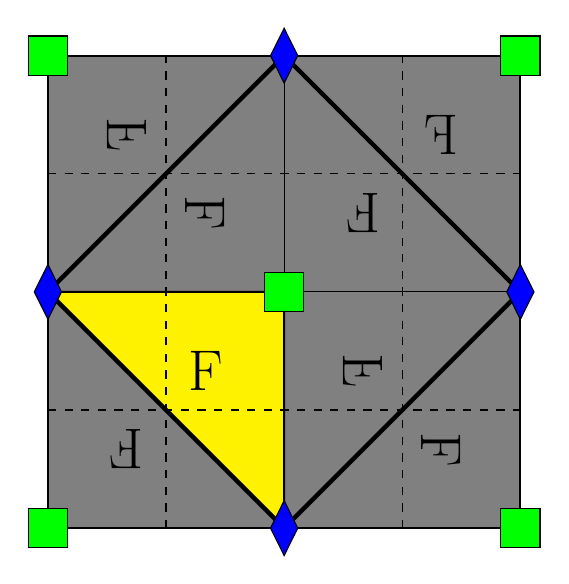
\begin{tikzpicture}
            % Define the lengths of the sides and the angle
            \def\a{3}  % length of side a
            \def\b{3}  % length of side b
            \def\angle{90}  % angle between sides a and b
            \def\s{F}
        
            % Calculate the coordinates of the points
            \coordinate (C00) at (0, 0);
            \coordinate (C10) at (\a, 0);
            \coordinate (C11) at ({\a + \b*cos(\angle)}, {\b * sin(\angle)});
            \coordinate (C01) at ({\b * cos(\angle)}, {\b * sin(\angle)});
            \coordinate (C02) at ({2*\b*cos(\angle)}, {2*\b * sin(\angle)});
            \coordinate (C12) at ({\a +2*\b * cos(\angle)}, {2*\b * sin(\angle)});
            \coordinate (C22) at ({2*\a + 2*\b * cos(\angle)}, {2*\b * sin(\angle)});
            \coordinate (C21) at ({2*\a + \b*cos(\angle)}, {\b * sin(\angle)});
            \coordinate (C20) at ({2*\a}, 0);
        
            % Draw the oblique unit cell
            \draw[thick,fill=gray] (C00) -- (C20) -- (C22) -- (C02) -- cycle;
            \draw[thick,fill=yellow] (C01) -- (C10) -- (C11) -- cycle;
            \draw[ultra thick] (C10) -- (C21) -- (C12) -- (C01) -- cycle;

            
            % Draw mirrow lines
            \draw[dashed] ($(C00)!0.5!(C10)$) -- ($(C02)!0.5!(C12)$);
            \draw[thin] (C10) -- (C12);
            \draw[dashed] ($(C10)!0.5!(C20)$) -- ($(C12)!0.5!(C22)$);
            \draw[dashed] ($(C00)!0.5!(C01)$) -- ($(C20)!0.5!(C21)$);
            \draw[thin] (C01) -- (C21);
            \draw[dashed] ($(C01)!0.5!(C02)$) -- ($(C21)!0.5!(C22)$);
            
            % Draw chiral center
            \node[rotate=180] at ($(C11)!0.6666!(C00)$) {\huge \s};
            \node at ($(C11)!0.3333!(C00)$) {\huge \s};
            \node[rotate=90] at ($(C11)!0.6666!(C02)$) {\reflectbox{\huge \s}};
            \node[rotate=-90] at ($(C11)!0.3333!(C02)$) {\huge \s};
            \node at ($(C11)!0.6666!(C22)$) {\reflectbox{\huge \s}};
            \node[rotate=180] at ($(C11)!0.3333!(C22)$) {\huge \s};
            \node[rotate=-90] at ($(C11)!0.6666!(C20)$) {\huge \s};
            \node[rotate=90] at ($(C11)!0.3333!(C20)$) {\reflectbox{\huge 
            \s}};

            % Draw node reflections
            \draw (C00)  node[minimum size=0.5cm,draw,fill=green] {};
            \draw (C10)  node[shape aspect=0.5,diamond,draw,fill=blue] {};
            \draw (C11)  node[minimum size=0.5cm,draw,fill=green] {};
            \draw (C01)  node[shape aspect=0.5,diamond,draw,fill=blue] {};
            \draw (C02)  node[minimum size=0.5cm,draw,fill=green] {};
            \draw (C12)  node[shape aspect=0.5,diamond,draw,fill=blue] {};
            \draw (C22)  node[minimum size=0.5cm,draw,fill=green] {};
            \draw (C21)  node[shape aspect=0.5,diamond,draw,fill=blue] {};
            \draw (C20)  node[minimum size=0.5cm,draw,fill=green] {};

            %\draw ($(A)!0.5!(E)$) node[shape aspect=0.5,diamond,draw,fill=black] {};
            
        \end{tikzpicture}
\end{document}
        \caption{p4g}
        \label{fig:p4g}
    \end{figure}
\end{frame}

\begin{frame}{CM Wallpaper Group}
    \begin{figure}
        \centering
        \documentclass[class=article, crop=false]{standalone}
\usepackage{tikz}
\usepackage{subcaption}
\usetikzlibrary{calc}
\usetikzlibrary {shapes.geometric}

\begin{document}
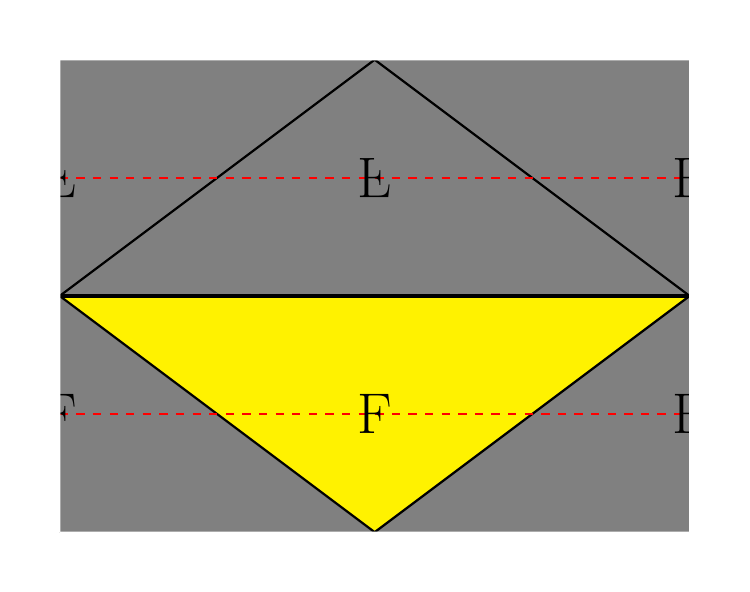
\begin{tikzpicture}
    % Define the lengths of the sides and the angle
    \def\a{4}  % length of side a
    \def\b{3}  % length of side b
    \def\angle{90}  % angle between sides a and b
    \def\s{F} % Label in center of cells

    \def\x{0.4}
    \def\y{0.4}

    % Calculate the coordinates of the points
    \coordinate (C00) at (0, 0);
    \coordinate (C10) at (\a, 0);
    \coordinate (C11) at ({\a + \b*cos(\angle)}, {\b * sin(\angle)});
    \coordinate (C01) at ({\b * cos(\angle)}, {\b * sin(\angle)});
    \coordinate (C02) at ({2*\b*cos(\angle)}, {2*\b * sin(\angle)});
    \coordinate (C12) at ({\a +2*\b * cos(\angle)}, {2*\b * sin(\angle)});
    \coordinate (C22) at ({2*\a + 2*\b * cos(\angle)}, {2*\b * sin(\angle)});
    \coordinate (C21) at ({2*\a + \b*cos(\angle)}, {\b * sin(\angle)});
    \coordinate (C20) at ({2*\a}, 0);

        
    % Draw the oblique unit cell
    \draw[fill=gray,gray] (C00) -- (C20) -- (C22) -- (C02) -- cycle;
    \draw[fill=yellow,yellow] (C10) -- (C21) -- (C01) -- cycle;

    % Draw mirror lines
    \draw[ultra thick] (C01) -- (C21);
    \draw[thick] (C10) -- (C21) -- (C12) -- (C01) -- cycle;
    \draw[thick,dashed,red] ($(C00)!0.5!(C01)$) -- ($(C20)!0.5!(C21)$);
    \draw[thick,dashed,red] ($(C01)!0.5!(C02)$) -- ($(C21)!0.5!(C22)$);

    

    % Draw boundary centre symbols
    \node at ($(C00)!0.5!(C01)$) {\huge \s};
    \node[rotate=180] at ($(C01)!0.5!(C02)$) {\reflectbox{\huge \s}};
    \node at ($(C20)!0.5!(C21)$) {\huge \s};
    \node[rotate=180] at ($(C21)!0.5!(C22)$) {\reflectbox{\huge \s}};

    % Create white border
    \draw[fill=white,white] ($(C00)-(\x,\y)$) -- ($(C20)-(-\x,\y)$) -- (C20) -- (C00);
    \draw[fill=white,white] ($(C00)-(\x,-\y)$) -- ($(C02)-(\x,-\y)$) -- (C02) -- (C00);
    \draw[fill=white,white] ($(C02)+(\x,\y)$) -- ($(C22)-(\x,-\y)$) -- (C22) -- (C02);
    \draw[fill=white,white] ($(C20)+(\x,-\y)$) -- ($(C22)+(\x,\y)$) -- (C22) -- (C20);
    
    % Center symbols
    \node at ($(C10)!0.5!(C11)$) {\huge \s};
    \node[rotate=180] at ($(C11)!0.5!(C12)$) {\reflectbox{\huge \s}};
    
\end{tikzpicture}
\end{document}
        \caption{cm}
        \label{fig:cm}
    \end{figure}
\end{frame}

\begin{frame}{CMM Wallpaper Group}
    \begin{figure}
        \centering
        \documentclass[class=article, crop=false]{standalone}
\usepackage{tikz}
\usepackage{subcaption}
\usetikzlibrary{calc}
\usetikzlibrary {shapes.geometric}

\begin{document}
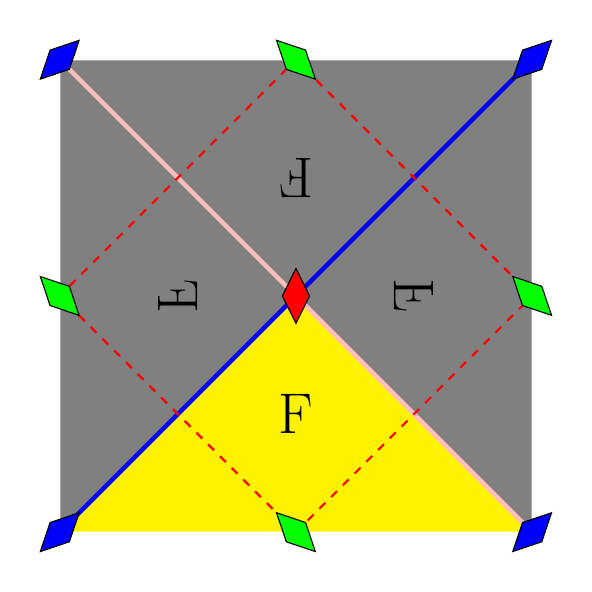
\begin{tikzpicture}
    % Define the lengths of the sides and the angle
    \def\a{3}  % length of side a
    \def\b{3}  % length of side b
    \def\angle{90}  % angle between sides a and b
    \def\s{F} % Label in center of cells

    \def\x{0.4}
    \def\y{0.4}

    % Calculate the coordinates of the points
    \coordinate (C00) at (0, 0);
    \coordinate (C10) at (\a, 0);
    \coordinate (C11) at ({\a + \b*cos(\angle)}, {\b * sin(\angle)});
    \coordinate (C01) at ({\b * cos(\angle)}, {\b * sin(\angle)});
    \coordinate (C02) at ({2*\b*cos(\angle)}, {2*\b * sin(\angle)});
    \coordinate (C12) at ({\a +2*\b * cos(\angle)}, {2*\b * sin(\angle)});
    \coordinate (C22) at ({2*\a + 2*\b * cos(\angle)}, {2*\b * sin(\angle)});
    \coordinate (C21) at ({2*\a + \b*cos(\angle)}, {\b * sin(\angle)});
    \coordinate (C20) at ({2*\a}, 0);

        
    % Draw the oblique unit cell
    \draw[fill=gray,gray] (C00) -- (C20) -- (C22) -- (C02) -- cycle;
    \draw[fill=yellow,yellow] (C00) -- (C11) -- (C20) -- cycle;

    % Draw mirror lines
    \draw[ultra thick,blue] (C00) -- (C22);
    \draw[ultra thick,pink] (C20) -- (C02);
    \draw[thick,dashed,red] (C10) -- (C21) -- (C12) -- (C01) -- cycle;
    
    

    % Draw boundary centre symbols
    %\node[rotate=180] at ($(C00)!0.5!(C01)$) {\huge \s};
    %\node[rotate=0] at ($(C01)!0.5!(C02)$) {\reflectbox{\huge \s}};
    %\node at ($(C20)!0.5!(C21)$) {\huge \s};
    %\node[rotate=180] at ($(C21)!0.5!(C22)$) {\reflectbox{\huge \s}};

    % Create white border
    \draw[fill=white,white] ($(C00)-(\x,\y)$) -- ($(C20)-(-\x,\y)$) -- (C20) -- (C00);
    \draw[fill=white,white] ($(C00)-(\x,-\y)$) -- ($(C02)-(\x,-\y)$) -- (C02) -- (C00);
    \draw[fill=white,white] ($(C02)+(\x,\y)$) -- ($(C22)-(\x,-\y)$) -- (C22) -- (C02);
    \draw[fill=white,white] ($(C20)+(\x,-\y)$) -- ($(C22)+(\x,\y)$) -- (C22) -- (C20);
    
    % Center symbols
    \node at ($(C10)!0.5!(C11)$) {\huge \s};
    \node[rotate=270] at ($(C01)!0.5!(C11)$) {\reflectbox{\huge \s}};
    \node[rotate=180] at ($(C12)!0.5!(C11)$) {\huge \s};
    \node[rotate=90] at ($(C21)!0.5!(C11)$) {\reflectbox{\huge \s}};

    % Draw node rotations
    \draw (C11)  node[rotate = 0,shape aspect=0.5,diamond,draw,fill=red] {};
    \draw (C10)  node[rotate = 45,shape aspect=0.5,diamond,draw,fill=green] {};
    \draw (C01)  node[rotate = 45,shape aspect=0.5,diamond,draw,fill=green] {};
    \draw (C21)  node[rotate = 45,shape aspect=0.5,diamond,draw,fill=green] {};
    \draw (C12)  node[rotate = 45,shape aspect=0.5,diamond,draw,fill=green] {};
    \draw (C00)  node[rotate = 135,shape aspect=0.5,diamond,draw,fill=blue] {};
    \draw (C20)  node[rotate = 135,shape aspect=0.5,diamond,draw,fill=blue] {};
    \draw (C02)  node[rotate = 135,shape aspect=0.5,diamond,draw,fill=blue] {};
    \draw (C22)  node[rotate = 135,shape aspect=0.5,diamond,draw,fill=blue] {};
    
\end{tikzpicture}
\end{document}
        \caption{cmm}
        \label{fig:cmm}
    \end{figure}
\end{frame}

\begin{frame}{PG Wallpaper Group}
    \begin{figure}
        \centering
        \documentclass[class=article, crop=false]{standalone}
\usepackage{tikz}
\usepackage{subcaption}
\usetikzlibrary{calc}
\usetikzlibrary {shapes.geometric}

\begin{document}
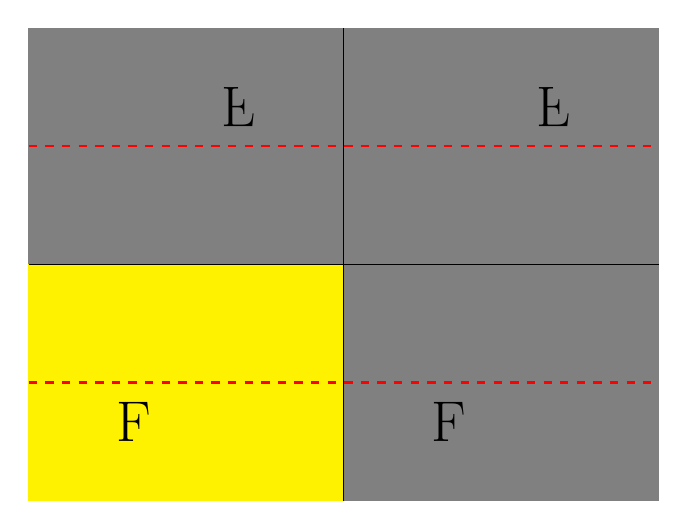
\begin{tikzpicture}
            % Define the lengths of the sides and the angle
            \def\a{4}  % length of side a
            \def\b{3}  % length of side b
            \def\angle{90}  % angle between sides a and b
            \def\s{F} % Label in center of cells


        
            % Calculate the coordinates of the points
            \coordinate (C00) at (0, 0);
            \coordinate (C10) at (\a, 0);
            \coordinate (C11) at ({\a + \b*cos(\angle)}, {\b * sin(\angle)});
            \coordinate (C01) at ({\b * cos(\angle)}, {\b * sin(\angle)});
            \coordinate (C02) at ({2*\b*cos(\angle)}, {2*\b * sin(\angle)});
            \coordinate (C12) at ({\a +2*\b * cos(\angle)}, {2*\b * sin(\angle)});
            \coordinate (C22) at ({2*\a + 2*\b * cos(\angle)}, {2*\b * sin(\angle)});
            \coordinate (C21) at ({2*\a + \b*cos(\angle)}, {\b * sin(\angle)});
            \coordinate (C20) at ({2*\a}, 0);

            \coordinate (A1) at ($(C00)!0.6666!(C11)$);
            \coordinate (A2) at ($(C11)!0.3333!(C22)$);
        
            % Draw the oblique unit cell
            \draw[fill=gray,gray] (C00) -- (C20) -- (C22) -- (C02) -- cycle;
            \draw[fill=yellow,yellow] (C00) -- (C01) -- (C11) -- (C10) -- cycle;
            \draw[] (C01) -- (C11) -- (C12);
            \draw[] (C10) -- (C11) -- (C21);
            
            % Draw chiral center
            \node at ($(C00)!0.3333!(C11)$) {\huge \s};
            \node at ($(C10)!0.3333!(C21)$) {\huge \s};
            \node[rotate=180] at ($(C11)!0.6666!(C22)$) {\reflectbox{\huge \s}};
            \node[rotate=180] at ($(C01)!0.6666!(C12)$) {\reflectbox{\huge \s}};

            % Draw mirror lines
            \draw[thick,dashed,red] ($(C00)!0.5!(C01)$) -- ($(C20)!0.5!(C21)$);
            \draw[thick,dashed,red] ($(C01)!0.5!(C02)$) -- ($(C21)!0.5!(C22)$);

            
        \end{tikzpicture}
\end{document}
        \caption{pg}
        \label{fig:pg}
    \end{figure}
\end{frame}

\begin{frame}{PGG Wallpaper Group}
    \begin{figure}
        \centering
        \documentclass[class=article, crop=false]{standalone}
\usepackage{tikz}
\usepackage{subcaption}
\usetikzlibrary{calc}
\usetikzlibrary {shapes.geometric}

\begin{document}
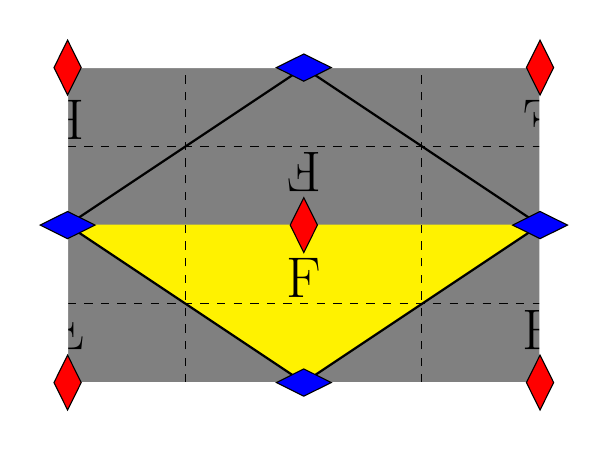
\begin{tikzpicture}
            % Define the lengths of the sides and the angle
            \def\a{3}  % length of side a
            \def\b{2}  % length of side b
            \def\angle{90}  % angle between sides a and b
            \def\s{F}

            \def\x{0.5} % Boundary 
            \def\y{0.5} % Boundary
        
            % Calculate the coordinates of the points
            \coordinate (C00) at (0, 0);
            \coordinate (C10) at (\a, 0);
            \coordinate (C11) at ({\a + \b*cos(\angle)}, {\b * sin(\angle)});
            \coordinate (C01) at ({\b * cos(\angle)}, {\b * sin(\angle)});
            \coordinate (C02) at ({2*\b*cos(\angle)}, {2*\b * sin(\angle)});
            \coordinate (C12) at ({\a +2*\b * cos(\angle)}, {2*\b * sin(\angle)});
            \coordinate (C22) at ({2*\a + 2*\b * cos(\angle)}, {2*\b * sin(\angle)});
            \coordinate (C21) at ({2*\a + \b*cos(\angle)}, {\b * sin(\angle)});
            \coordinate (C20) at ({2*\a}, 0);
        
            % Draw the oblique unit cell
            \draw[fill=gray,gray] (C00) -- (C20) -- (C22) -- (C02) -- cycle;
            \draw[fill=yellow,yellow] (C01) -- (C10) -- (C21) -- cycle;
            \draw[thick] (C10) -- (C21) -- (C12) -- (C01) -- cycle;
            
            % Draw mirrow lines
            \draw[dashed] ($(C00)!0.5!(C01)$) -- ($(C20)!0.5!(C21)$);
            \draw[dashed] ($(C01)!0.5!(C02)$) -- ($(C21)!0.5!(C22)$);
            \draw[dashed] ($(C00)!0.5!(C10)$) -- ($(C02)!0.5!(C12)$);
            \draw[dashed] ($(C10)!0.5!(C20)$) -- ($(C12)!0.5!(C22)$);


            % Draw inner centres
            \node at ($(C01)!0.6666!(C02)$) {\reflectbox{\huge \s}};
            \node[rotate=180] at ($(C00)!0.3333!(C01)$) {\reflectbox{\huge \s}};
            \node at ($(C21)!0.6666!(C22)$) {\reflectbox{\huge \s}};
            \node[rotate=180] at ($(C20)!0.3333!(C21)$) {\reflectbox{\huge \s}};

            % Create white border
            \draw[fill=white,white] ($(C00)-(\x,\y)$) -- ($(C20)-(-\x,\y)$) -- (C20) -- (C00);
            \draw[fill=white,white] ($(C00)-(\x,-\y)$) -- ($(C02)-(\x,-\y)$) -- (C02) -- (C00);
            \draw[fill=white,white] ($(C02)+(\x,\y)$) -- ($(C22)-(\x,-\y)$) -- (C22) -- (C02);
            \draw[fill=white,white] ($(C20)+(\x,-\y)$) -- ($(C22)+(\x,\y)$) -- (C22) -- (C20);
            
            % Draw chiral center
            \node at ($(C10)!0.6666!(C11)$) {\huge \s};
            \node[rotate=180] at ($(C11)!0.3333!(C12)$) {\huge \s};
            

            % Draw node reflections
            \draw (C00)  node[shape aspect=0.5,diamond,draw,fill=red] {};
            \draw (C10)  node[shape aspect=0.5,rotate=90,diamond,draw,fill=blue] {};
            \draw (C11)  node[shape aspect=0.5,diamond,draw,fill=red] {};
            \draw (C01)  node[shape aspect=0.5,rotate=90,diamond,draw,fill=blue] {};
            \draw (C02)  node[shape aspect=0.5,diamond,draw,fill=red] {};
            \draw (C12)  node[shape aspect=0.5,rotate=90,diamond,draw,fill=blue] {};
            \draw (C22)  node[shape aspect=0.5,diamond,draw,fill=red] {};
            \draw (C21)  node[shape aspect=0.5,rotate=90,diamond,draw,fill=blue] {};
            \draw (C20)  node[shape aspect=0.5,diamond,draw,fill=red] {};
        \end{tikzpicture}
\end{document}
        \caption{pgg}
        \label{fig:pgg}
    \end{figure}
\end{frame}

\begin{frame}{PMG Wallpaper Group}
    \begin{figure}
        \centering
        \documentclass[class=article, crop=false]{standalone}
\usepackage{tikz}
\usepackage{subcaption}
\usetikzlibrary{calc}
\usetikzlibrary {shapes.geometric}

\begin{document}
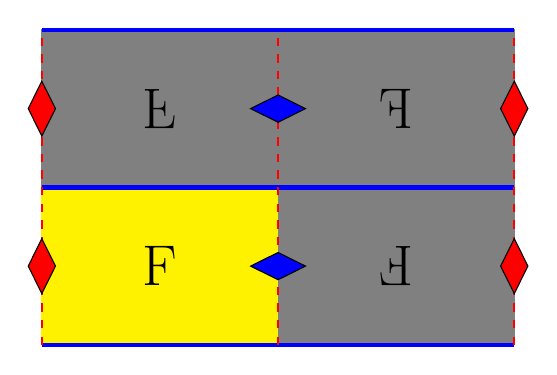
\begin{tikzpicture}
            % Define the lengths of the sides and the angle
            \def\a{3}  % length of side a
            \def\b{2}  % length of side b
            \def\angle{90}  % angle between sides a and b
            \def\s{F}
        
            % Calculate the coordinates of the points
            \coordinate (C00) at (0, 0);
            \coordinate (C10) at (\a, 0);
            \coordinate (C11) at ({\a + \b*cos(\angle)}, {\b * sin(\angle)});
            \coordinate (C01) at ({\b * cos(\angle)}, {\b * sin(\angle)});
            \coordinate (C02) at ({2*\b*cos(\angle)}, {2*\b * sin(\angle)});
            \coordinate (C12) at ({\a +2*\b * cos(\angle)}, {2*\b * sin(\angle)});
            \coordinate (C22) at ({2*\a + 2*\b * cos(\angle)}, {2*\b * sin(\angle)});
            \coordinate (C21) at ({2*\a + \b*cos(\angle)}, {\b * sin(\angle)});
            \coordinate (C20) at ({2*\a}, 0);
        
            % Draw the oblique unit cell
            \draw[fill=yellow,yellow] (C00) -- (C01) -- (C11) -- (C10) -- cycle;
            \draw[fill=gray,gray] (C01) -- (C11) -- (C12) -- (C02) -- cycle;
            
            \draw[fill=gray,gray] (C11) -- (C12) -- (C22) -- (C21) -- cycle;
            \draw[fill=gray,gray] (C10) -- (C20) -- (C21) -- (C11) -- cycle;

            % Draw mirror lines
            \draw[ultra thick,blue] (C00) -- (C20);
            \draw[ultra thick,blue] (C01) -- (C21);
            \draw[ultra thick,blue] (C02) -- (C22);
            \draw[thick,dashed,red] (C00) -- (C02);
            \draw[thick,dashed,red] (C10) -- (C12);
            \draw[thick,dashed,red] (C20) -- (C22);
            
            % Draw chiral center
            \node at ($(C00)!0.5!(C11)$) {\huge \s};
            \node[rotate=180] at ($(C01)!0.5!(C12)$) {\reflectbox{\huge \s}};
            \node[rotate=180] at ($(C10)!0.5!(C21)$) {\huge \s};
            \node[rotate=0] at ($(C11)!0.5!(C22)$) {\reflectbox{\huge \s}};

            % Draw node rotations
            \draw ($(C00)!0.5!(C01)$)  node[shape aspect=0.5,diamond,draw,fill=red] {};
            \draw ($(C01)!0.5!(C02)$)  node[shape aspect=0.5,diamond,draw,fill=red] {};
            \draw ($(C10)!0.5!(C11)$)  node[rotate = 90,shape aspect=0.5,diamond,draw,fill=blue] {};
            \draw ($(C11)!0.5!(C12)$)  node[shape aspect=0.5,rotate=90,diamond,draw,fill=blue] {};
            \draw ($(C20)!0.5!(C21)$)  node[shape aspect=0.5,diamond,draw,fill=red] {};
            \draw ($(C21)!0.5!(C22)$)  node[shape aspect=0.5,diamond,draw,fill=red] {};
            
        \end{tikzpicture}
\end{document}
        \caption{pmg}
        \label{fig:pmg}
    \end{figure}
\end{frame}

\begin{frame}{PM Wallpaper Group}
    \begin{figure}
        \centering
        \documentclass[class=article, crop=false]{standalone}
\usepackage{tikz}
\usepackage{subcaption}
\usetikzlibrary{calc}
\usetikzlibrary {shapes.geometric}

\begin{document}
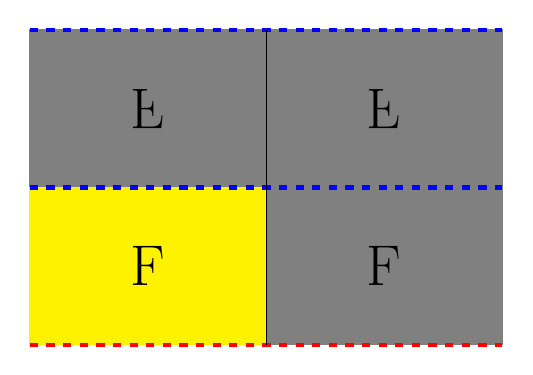
\begin{tikzpicture}
            % Define the lengths of the sides and the angle
            \def\a{3}  % length of side a
            \def\b{2}  % length of side b
            \def\angle{90}  % angle between sides a and b
            \def\s{F} % Label in center of cells

            \def\x{0.5} % Boundary 
            \def\y{0.5} % Boundary
        
            % Calculate the coordinates of the points
            \coordinate (C00) at (0, 0);
            \coordinate (C10) at (\a, 0);
            \coordinate (C11) at ({\a + \b*cos(\angle)}, {\b * sin(\angle)});
            \coordinate (C01) at ({\b * cos(\angle)}, {\b * sin(\angle)});
            \coordinate (C02) at ({2*\b*cos(\angle)}, {2*\b * sin(\angle)});
            \coordinate (C12) at ({\a +2*\b * cos(\angle)}, {2*\b * sin(\angle)});
            \coordinate (C22) at ({2*\a + 2*\b * cos(\angle)}, {2*\b * sin(\angle)});
            \coordinate (C21) at ({2*\a + \b*cos(\angle)}, {\b * sin(\angle)});
            \coordinate (C20) at ({2*\a}, 0);

            \coordinate (A1) at ($(C00)!0.6666!(C11)$);
            \coordinate (A2) at ($(C11)!0.3333!(C22)$);
        
            % Draw the oblique unit cell
            \draw[fill=gray,gray] (C00) -- (C20) -- (C22) -- (C02) -- cycle;
            \draw[fill=yellow,yellow] (C00) -- (C10) -- (C11) -- (C01) -- cycle;


            % Draw mirror lines
            \draw[ultra thick,blue,dashed] (C01) -- (C21);
            \draw[ultra thick,red,dashed] (C00) -- (C20);
            \draw[ultra thick,blue,dashed] (C02) -- (C22);
            \draw[] (C10) -- (C12);
            
           
            
            % Draw chiral center
            \node at ($(C00)!0.5!(C11)$) {\huge F};
            \node[rotate=180] at ($(C01)!0.5!(C12)$) {\reflectbox{\huge F}};
            \node at ($(C10)!0.5!(C21)$) {\huge F};
            \node[rotate=180] at ($(C11)!0.5!(C22)$) {\reflectbox{\huge F}};

            
        \end{tikzpicture}
\end{document}
        \caption{pm}
        \label{fig:pmm}
    \end{figure}
\end{frame}

\begin{frame}{PMM Wallpaper Group}
    \begin{figure}
        \centering
        \documentclass[class=article, crop=false]{standalone}
\usepackage{tikz}
\usepackage{subcaption}
\usetikzlibrary{calc}
\usetikzlibrary {shapes.geometric}

\begin{document}
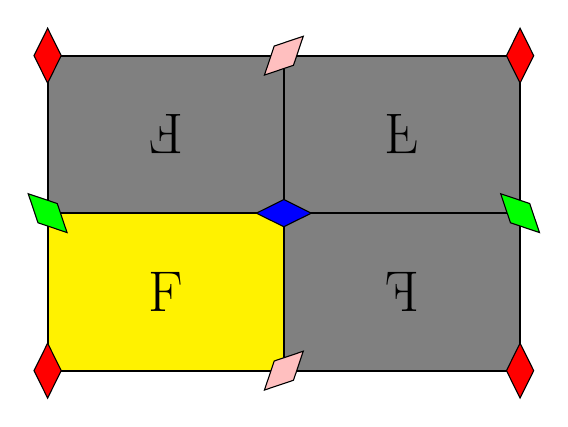
\begin{tikzpicture}
            % Define the lengths of the sides and the angle
            \def\a{3}  % length of side a
            \def\b{2}  % length of side b
            \def\angle{90}  % angle between sides a and b
            \def\s{F}

        
            % Calculate the coordinates of the points
            \coordinate (C00) at (0, 0);
            \coordinate (C10) at (\a, 0);
            \coordinate (C11) at ({\a + \b*cos(\angle)}, {\b * sin(\angle)});
            \coordinate (C01) at ({\b * cos(\angle)}, {\b * sin(\angle)});
            \coordinate (C02) at ({2*\b*cos(\angle)}, {2*\b * sin(\angle)});
            \coordinate (C12) at ({\a +2*\b * cos(\angle)}, {2*\b * sin(\angle)});
            \coordinate (C22) at ({2*\a + 2*\b * cos(\angle)}, {2*\b * sin(\angle)});
            \coordinate (C21) at ({2*\a + \b*cos(\angle)}, {\b * sin(\angle)});
            \coordinate (C20) at ({2*\a}, 0);
        
            % Draw the oblique unit cell
            \draw[thick,fill=yellow] (C00) -- (C01) -- (C11) -- (C10) -- cycle;
            \draw[thick,fill=gray] (C01) -- (C11) -- (C12) -- (C02) -- cycle;
            
            \draw[thick,fill=gray] (C11) -- (C12) -- (C22) -- (C21) -- cycle;
            \draw[thick,fill=gray] (C10) -- (C20) -- (C21) -- (C11) -- cycle;
            
            % Draw chiral center
            \node at ($(C00)!0.5!(C11)$) {\huge \s};
            \node[rotate=180] at ($(C01)!0.5!(C12)$) {\huge \s};
            \node at ($(C10)!0.5!(C21)$) {\reflectbox{\huge \s}};
            \node[rotate=180] at ($(C11)!0.5!(C22)$) {\reflectbox{\huge \s}};

            % Draw node reflections
            \draw (C00)  node[shape aspect=0.5,diamond,draw,fill=red] {};
            \draw (C10)  node[shape aspect=0.5,rotate=-45,diamond,draw,fill=pink] {};
            \draw (C11)  node[rotate = \angle,shape aspect=0.5,diamond,draw,fill=blue] {};
            \draw (C01)  node[shape aspect=0.5,rotate=45,diamond,draw,fill=green] {};
            \draw (C02)  node[shape aspect=0.5,diamond,draw,fill=red] {};
            \draw (C12)  node[shape aspect=0.5,rotate=-45,diamond,draw,fill=pink] {};
            \draw (C22)  node[shape aspect=0.5,diamond,draw,fill=red] {};
            \draw (C21)  node[shape aspect=0.5,rotate=45,diamond,draw,fill=green] {};
            \draw (C20)  node[shape aspect=0.5,diamond,draw,fill=red] {};

            %\draw ($(A)!0.5!(E)$) node[shape aspect=0.5,diamond,draw,fill=black] {};
            
        \end{tikzpicture}
\end{document}
        \caption{pmm}
        \label{fig:pmm}
    \end{figure}
\end{frame}

\begin{frame}{P3 Wallpaper Group}
    \begin{figure}
        \centering
        \documentclass[class=article, crop=false]{standalone}
\usepackage{tikz}
\usepackage{subcaption}
\usetikzlibrary{calc}
\usetikzlibrary {shapes.geometric}

\begin{document}
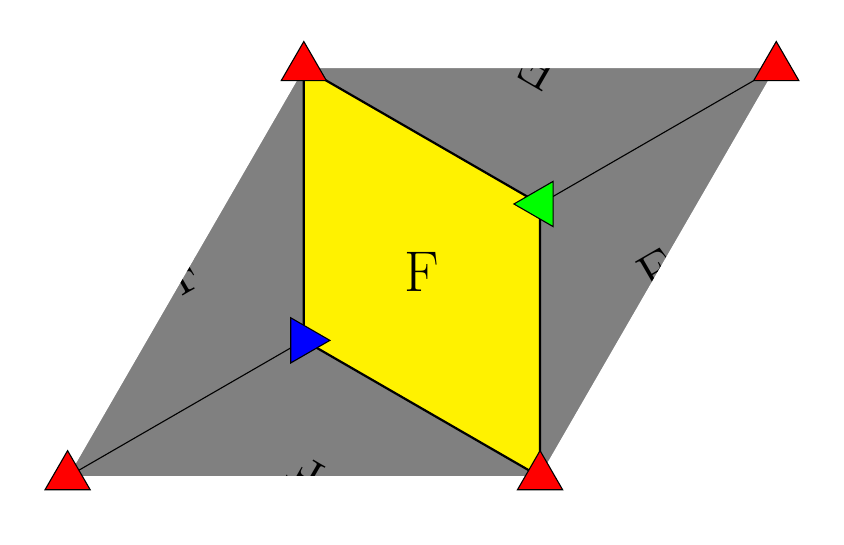
\begin{tikzpicture}
            % Define the lengths of the sides and the angle
            \def\a{3}  % length of side a
            \def\b{3}  % length of side b
            \def\angle{60}  % angle between sides a and b
            \def\s{F} % Label in center of cells

            \def\x{0.5} % Boundary 
            \def\y{0.5} % Boundary

        
            % Calculate the coordinates of the points
            \coordinate (C00) at (0, 0);
            \coordinate (C10) at (\a, 0);
            \coordinate (C11) at ({\a + \b*cos(\angle)}, {\b * sin(\angle)});
            \coordinate (C01) at ({\b * cos(\angle)}, {\b * sin(\angle)});
            \coordinate (C02) at ({2*\b*cos(\angle)}, {2*\b * sin(\angle)});
            \coordinate (C12) at ({\a +2*\b * cos(\angle)}, {2*\b * sin(\angle)});
            \coordinate (C22) at ({2*\a + 2*\b * cos(\angle)}, {2*\b * sin(\angle)});
            \coordinate (C21) at ({2*\a + \b*cos(\angle)}, {\b * sin(\angle)});
            \coordinate (C20) at ({2*\a}, 0);
        
            % Draw the oblique unit cell
            \draw[fill=gray,gray] (C00) -- (C20) -- (C22) -- (C02) -- cycle;
            \draw[thick,fill=yellow] ($(C00)!0.6666!(C11)$) -- (C20) -- ($(C11)!0.3333!(C22)$) -- (C02) -- cycle;

            
            % Draw boundary chiral centres
            \node[rotate=150] at (C10) {\huge \s};
            \node[rotate=30] at (C21) {\huge \s};
            \node[rotate=150] at (C12) {\huge \s};
            \node[rotate=30] at (C01) {\huge \s};

            % Create white border
            \draw[fill=white,white] ($(C00)-(\x,\y)$) -- ($(C20)-(-\x,\y)$) -- (C20) -- (C00);
            \draw[fill=white,white] ($(C00)-(\x,-\y)$) -- ($(C02)-(\x,-\y)$) -- (C02) -- (C00);
            \draw[fill=white,white] ($(C02)+(\x,\y)$) -- ($(C22)-(\x,-\y)$) -- (C22) -- (C02);
            \draw[fill=white,white] ($(C20)+(\x,-\y)$) -- ($(C22)+(\x,\y)$) -- (C22) -- (C20);

            % Draw chiral inner centre
            \node at (C11) {\huge \s};


            % Draw mirrow lines
            \draw (C00) -- ($(C00)!0.6666!(C11)$);
            \draw ($(C11)!0.3333!(C22)$) -- (C22);


            % Draw node reflections
            \draw (C00)  node[regular polygon, regular polygon sides=3, draw, fill=red, minimum size=0.5cm] {};
            \draw (C02)  node[regular polygon, regular polygon sides=3, draw, fill=red, minimum size=0.5cm] {};
            \draw (C22)  node[regular polygon, regular polygon sides=3, draw, fill=red, minimum size=0.5cm] {};
            \draw (C20)  node[regular polygon, regular polygon sides=3, draw, fill=red, minimum size=0.5cm] {};

            \draw ($(C00)!0.6666!(C11)$)  node[rotate = 30,regular polygon, regular polygon sides=3, draw, fill=blue, minimum size=0.5cm] {};
            \draw ($(C11)!0.3333!(C22)$)  node[rotate=90, regular polygon, regular polygon sides=3, draw, fill=green, minimum size=0.5cm] {};    
        \end{tikzpicture}
\end{document}
        \caption{p3}
        \label{fig:p3}
    \end{figure}
\end{frame}

\begin{frame}{P3M1 Wallpaper Group}
    \begin{figure}
        \centering
        \documentclass[class=article, crop=false]{standalone}
\usepackage{tikz}
\usepackage{subcaption}
\usetikzlibrary{calc}
\usetikzlibrary {shapes.geometric}

\begin{document}
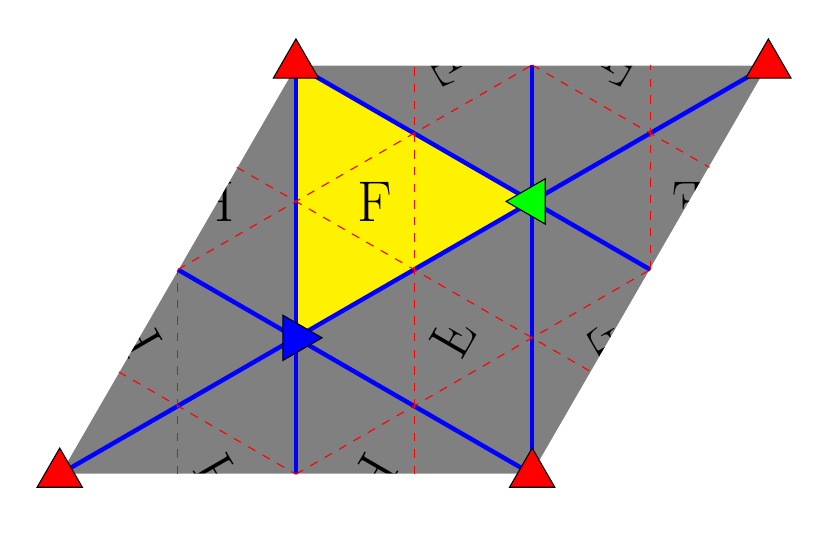
\begin{tikzpicture}
            % Define the lengths of the sides and the angle
            \def\a{3}  % length of side a
            \def\b{3}  % length of side b
            \def\angle{60}  % angle between sides a and b
            \def\s{F} % Label in center of cells

            \def\x{0.4}
            \def\y{0.4}
        
            % Calculate the coordinates of the points
            \coordinate (C00) at (0, 0);
            \coordinate (C10) at (\a, 0);
            \coordinate (C11) at ({\a + \b*cos(\angle)}, {\b * sin(\angle)});
            \coordinate (C01) at ({\b * cos(\angle)}, {\b * sin(\angle)});
            \coordinate (C02) at ({2*\b*cos(\angle)}, {2*\b * sin(\angle)});
            \coordinate (C12) at ({\a +2*\b * cos(\angle)}, {2*\b * sin(\angle)});
            \coordinate (C22) at ({2*\a + 2*\b * cos(\angle)}, {2*\b * sin(\angle)});
            \coordinate (C21) at ({2*\a + \b*cos(\angle)}, {\b * sin(\angle)});
            \coordinate (C20) at ({2*\a}, 0);
            \coordinate (A1) at ($(C00)!0.6666!(C11)$);
            \coordinate (A2) at ($(C11)!0.3333!(C22)$);
        

            % Draw the oblique unit cell
            \draw[thick,fill=gray,gray] (C00) -- (C20) -- (C22) -- (C02) -- cycle;
            \draw[thick,fill=yellow,yellow] (A1) -- (A2) -- (C02) -- cycle;
            %\draw[thick] (C10) -- (C21) -- (C12) -- (C01) -- cycle;
            

            % Draw bourdary chiral centres
            \node[rotate=240] at ($(C10)!0.3333!(C20)$) {\huge \s};
            \node[rotate=120] at ($(C00)!0.6666!(C10)$) {\reflectbox{\huge \s}};
            \node[rotate=120] at ($(C00)!0.6666!(C01)$) {\huge \s};
            \node at ($(C01)!0.3333!(C02)$) {\reflectbox{\huge \s}};
            \node[rotate=120] at ($(C02)!0.6666!(C12)$) {\reflectbox{\huge \s}};
            \node[rotate=240] at ($(C12)!0.3333!(C22)$) {\huge \s};
            \node[rotate=120] at ($(C20)!0.6666!(C21)$) {\huge \s};
            \node at ($(C21)!0.3333!(C22)$) {\reflectbox{\huge \s}};

            % Create white border
            \draw[fill=white,white] ($(C00)-(\x,\y)$) -- ($(C20)-(-\x,\y)$) -- (C20) -- (C00);
            \draw[fill=white,white] ($(C00)-(\x,-\y)$) -- ($(C02)-(\x,-\y)$) -- (C02) -- (C00);
            \draw[fill=white,white] ($(C02)+(\x,\y)$) -- ($(C22)-(\x,-\y)$) -- (C22) -- (C02);
            \draw[fill=white,white] ($(C20)+(\x,-\y)$) -- ($(C22)+(\x,\y)$) -- (C22) -- (C20);

            % Draw inner chiral centres
            \node at ($(A1)!0.5!(A2)!0.3333!(C02)$) {\huge \s};
            \node[rotate=240] at ($(A1)!0.5!(A2)!0.3333!(C20)$) {\reflectbox{\huge \s}};

        

            % Draw mirrow lines
            \draw[ultra thick,blue] (C00)--(C22);
            \draw[ultra thick,blue] (C01)--(C20);
            \draw[ultra thick,blue] (C10)--(C02);
            \draw[ultra thick,blue] (C12)--(C20);
            \draw[ultra thick,blue] (C02)--(C21);
            \draw[dashed,red] ($(C00)!0.5!(C10)$)--(C01);
            \draw[dashed,red] ($(C00)!0.5!(C01)$)--(C10);
            \draw[dashed,red] ($(C10)!0.5!(C20)$)--($(C02)!0.5!(C12)$);
            \draw[dashed,red] ($(C01)!0.5!(C02)$)--($(C20)!0.5!(C21)$);
            \draw[dashed,red] (C01)--(C12);
            \draw[dashed,red] (C10)--(C21);
            \draw[dashed,red] (C12)--($(C21)!0.5!(C22)$);
            \draw[dashed,red] (C21)--($(C12)!0.5!(C22)$);
            

            

            % Draw node reflections
            \draw (C00)  node[regular polygon, regular polygon sides=3, draw, fill=red, minimum size=0.5cm] {};
            %\draw (C10)  node[shape aspect=0.5,rotate=90,diamond,draw,fill=blue] {};
            %\draw (C11)  node[shape aspect=0.5,diamond,draw,fill=red] {};
            %\draw (C01)  node[shape aspect=0.5,rotate=90,diamond,draw,fill=blue] {};
            \draw (C02)  node[regular polygon, regular polygon sides=3, draw, fill=red, minimum size=0.5cm] {};
            %\draw (C12)  node[shape aspect=0.5,rotate=90,diamond,draw,fill=blue] {};
            \draw (C22)  node[regular polygon, regular polygon sides=3, draw, fill=red, minimum size=0.5cm] {};
            %\draw (C21)  node[shape aspect=0.5,rotate=90,diamond,draw,fill=blue] {};
            \draw (C20)  node[regular polygon, regular polygon sides=3, draw, fill=red, minimum size=0.5cm] {};

            \draw (A1)  node[rotate = 30,regular polygon, regular polygon sides=3, draw, fill=blue, minimum size=0.5cm] {};
            \draw (A2)  node[rotate=90, regular polygon, regular polygon sides=3, draw, fill=green, minimum size=0.5cm] {};

            %\draw ($(A)!0.5!(E)$) node[shape aspect=0.5,diamond,draw,fill=black] {};
            
        \end{tikzpicture}
\end{document}
        \caption{p3m1}
        \label{fig:p3m1}
    \end{figure}
\end{frame}

\begin{frame}{P31M Wallpaper Group}
    \begin{figure}
        \centering
        \documentclass[class=article, crop=false]{standalone}
\usepackage{tikz}
\usepackage{subcaption}
\usetikzlibrary{calc}
\usetikzlibrary {shapes.geometric}

\begin{document}
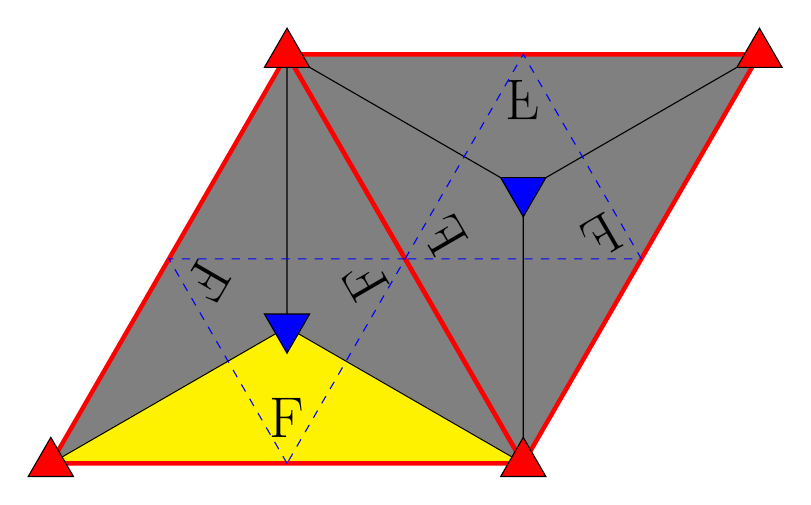
\begin{tikzpicture}
            % Define the lengths of the sides and the angle
            \def\a{3}  % length of side a
            \def\b{3}  % length of side b
            \def\angle{60}  % angle between sides a and b
            \def\s{F} % Label in center of cells

            \def\x{0.5} % Boundary 
            \def\y{0.5} % Boundary
        
            % Calculate the coordinates of the points
            \coordinate (C00) at (0, 0);
            \coordinate (C10) at (\a, 0);
            \coordinate (C11) at ({\a + \b*cos(\angle)}, {\b * sin(\angle)});
            \coordinate (C01) at ({\b * cos(\angle)}, {\b * sin(\angle)});
            \coordinate (C02) at ({2*\b*cos(\angle)}, {2*\b * sin(\angle)});
            \coordinate (C12) at ({\a +2*\b * cos(\angle)}, {2*\b * sin(\angle)});
            \coordinate (C22) at ({2*\a + 2*\b * cos(\angle)}, {2*\b * sin(\angle)});
            \coordinate (C21) at ({2*\a + \b*cos(\angle)}, {\b * sin(\angle)});
            \coordinate (C20) at ({2*\a}, 0);

            \coordinate (A1) at ($(C00)!0.6666!(C11)$);
            \coordinate (A2) at ($(C11)!0.3333!(C22)$);
        
            % Draw the oblique unit cell
            \draw[fill=gray,gray] (C00) -- (C20) -- (C22) -- (C02) -- cycle;
            \draw[fill=yellow,yellow] (C00) -- (A1) -- (C20) -- cycle;
            
            
            
            % Draw chiral center
            \node at ($(C00)!0.5!(C20)!0.3333!(A1)$) {\huge \s};
            \node[rotate=240] at ($(C00)!0.5!(C02)!0.3333!(A1)$) {\huge \s};
            \node[rotate=120] at ($(C20)!0.5!(C02)!0.3333!(A1)$) {\huge \s};
            \node[rotate=300] at ($(C20)!0.5!(C02)!0.3333!(A2)$) {\reflectbox{\huge \s}};
            \node[rotate=30] at ($(C20)!0.5!(C22)!0.3333!(A2)$) {\reflectbox{\huge \s}};
            \node[rotate=180] at ($(C02)!0.5!(C22)!0.3333!(A2)$) {\reflectbox{\huge \s}};

            % Draw mirrow lines
            \draw[ultra thick,red] (C00) -- (C02) -- (C20) -- cycle;
            \draw[ultra thick,red] (C02) -- (C22) -- (C20) -- cycle;
            \draw[thin] (C00) -- (A1) -- (C02) -- (A2) -- (C22);
            \draw[thin] (A1) -- (C20) -- (A2);
            \draw[dashed,blue] (C10) -- (C01) -- (C11) -- cycle;
            \draw[dashed,blue] (C11) -- (C12) -- (C21) -- cycle;
            

            % Draw node rotations symbols
            \draw (C00)  node[regular polygon, regular polygon sides=3, draw, fill=red, minimum size=0.5cm] {};
            \draw (C02)  node[regular polygon, regular polygon sides=3, draw, fill=red, minimum size=0.5cm] {};
            \draw (C22)  node[regular polygon, regular polygon sides=3, draw, fill=red, minimum size=0.5cm] {};
            \draw (C20)  node[regular polygon, regular polygon sides=3, draw, fill=red, minimum size=0.5cm] {};

            \draw (A1)  node[rotate = 180,regular polygon, regular polygon sides=3, draw, fill=blue, minimum size=0.5cm] {};
            \draw (A2)  node[rotate=180, regular polygon, regular polygon sides=3, draw, fill=blue, minimum size=0.5cm] {};

        \end{tikzpicture}
\end{document}
        \caption{p31m}
        \label{fig:p31m}
    \end{figure}
\end{frame}

\begin{frame}{P6 Wallpaper Group}
    \begin{figure}
        \centering
        \documentclass[class=article, crop=false]{standalone}
\usepackage{tikz}
\usepackage{subcaption}
\usetikzlibrary{calc}
\usetikzlibrary {shapes.geometric}

\begin{document}
\begin{tikzpicture}
            % Define the lengths of the sides and the angle
            \def\a{3}  % length of side a
            \def\b{3}  % length of side b
            \def\angle{60}  % angle between sides a and b
            \def\s{F} % Label in center of cells
        
            % Calculate the coordinates of the points
            \coordinate (C00) at (0, 0);
            \coordinate (C10) at (\a, 0);
            \coordinate (C11) at ({\a + \b*cos(\angle)}, {\b * sin(\angle)});
            \coordinate (C01) at ({\b * cos(\angle)}, {\b * sin(\angle)});
            \coordinate (C02) at ({2*\b*cos(\angle)}, {2*\b * sin(\angle)});
            \coordinate (C12) at ({\a +2*\b * cos(\angle)}, {2*\b * sin(\angle)});
            \coordinate (C22) at ({2*\a + 2*\b * cos(\angle)}, {2*\b * sin(\angle)});
            \coordinate (C21) at ({2*\a + \b*cos(\angle)}, {\b * sin(\angle)});
            \coordinate (C20) at ({2*\a}, 0);

            \coordinate (A1) at ($(C00)!0.6666!(C11)$);
            \coordinate (A2) at ($(C11)!0.3333!(C22)$);
        
            % Draw the oblique unit cell
            \draw[thick,fill=gray] (C00) -- (C20) -- (C22) -- (C02) -- cycle;
            \draw[thick,fill=yellow] (C00) -- (A1) -- (C20) -- cycle;
            %\draw[thick] (C10) -- (C21) -- (C12) -- (C01) -- cycle;
            
            % Draw mirrow lines
            \draw[thin] (C02) -- (A1);
            \draw[thin] (C02) -- (C11) -- (C20);
            \draw[thin] (C02) -- (A2) -- (C20);
            \draw[thin] (A2) -- (C22);
            
            % Draw chiral center
            $\node at ($(C00)!0.5!(C20)!0.5!(A1)$) {\huge \s};
            \node[rotate=240] at ($(C00)!0.5!(C02)!0.5!(A1)$) {\huge \s};
            \node[rotate=120] at ($(C20)!0.5!(C02)!0.5!(A1)$) {\huge \s};
            \node[rotate=300] at ($(C20)!0.5!(C02)!0.5!(A2)$) {\huge \s};
            \node[rotate=60] at ($(C22)!0.5!(C20)!0.5!(A2)$) {\huge \s};
            \node[rotate=180] at ($(C02)!0.5!(C22)!0.5!(A2)$) {\huge \s};

            % Draw node rotations
            \draw (C00)  node[regular polygon, regular polygon sides=6, draw, fill=blue, minimum size=0.5cm] {};
            \draw (C10)  node[shape aspect=0.5,diamond,draw,fill=black] {};
            \draw (C21)  node[shape aspect=0.5,diamond,draw,fill=black] {};
            \draw (C01)  node[shape aspect=0.5,diamond,draw,fill=black] {};
            \draw (C12)  node[shape aspect=0.5,diamond,draw,fill=black] {};
            \draw (C02)  node[regular polygon, regular polygon sides=6, draw, fill=blue, minimum size=0.5cm] {};
            %\draw (C12)  node[shape aspect=0.5,rotate=90,diamond,draw,fill=blue] {};
            \draw (C22)  node[regular polygon, regular polygon sides=6, draw, fill=blue, minimum size=0.5cm] {};
            %\draw (C21)  node[shape aspect=0.5,rotate=90,diamond,draw,fill=blue] {};
            \draw (C20)  node[regular polygon, regular polygon sides=6, draw, fill=blue, minimum size=0.5cm] {};

            \draw (A1)  node[regular polygon, regular polygon sides=3, draw, fill=red, minimum size=0.5cm] {};
            \draw (A2)  node[regular polygon, regular polygon sides=3, draw, fill=red, minimum size=0.5cm] {};

            \draw (C11) node[shape aspect=0.5,diamond,draw,fill=black] {};
            
        \end{tikzpicture}
\end{document}
        \caption{p6}
        \label{fig:p3}
    \end{figure}
\end{frame}

\begin{frame}{P6M Wallpaper Group}
    \begin{figure}
        \centering
        \documentclass[class=article, crop=false]{standalone}
\usepackage{tikz}
\usepackage{subcaption}
\usetikzlibrary{calc}
\usetikzlibrary {shapes.geometric}

\begin{document}
\begin{tikzpicture}
    % Define the lengths of the sides and the angle
    \def\a{3}  % length of side a
    \def\b{3}  % length of side b
    \def\angle{60}  % angle between sides a and b
    \def\s{T} % Label in center of cells

    % Calculate the coordinates of the points
    \coordinate (C00) at (0, 0);
g10) at (\a, 0);
    \coordinate (C11) at ({\a + \b*cos(\angle)}, {\b * sin(\angle)});
    \coordinate (C01) at ({\b * cos(\angle)}, {\b * sin(\angle)});
    \coordinate (C02) at ({2*\b*cos(\angle)}, {2*\b * sin(\angle)});
    \coordinate (C12) at ({\a +2*\b * cos(\angle)}, {2*\b * sin(\angle)});
    \coordinate (C22) at ({2*\a + 2*\b * cos(\angle)}, {2*\b * sin(\angle)});
    \coordinate (C21) at ({2*\a + \b*cos(\angle)}, {\b * sin(\angle)});
    \coordinate (C20) at ({2*\a}, 0);

    \coordinate (A1) at ($(C00)!0.6666!(C11)$);
    \coordinate (A2) at ($(C11)!0.3333!(C22)$);

    % Draw the oblique unit cell
    \draw[fill=gray] (C00) -- (C20) -- (C22) -- (C02) -- cycle;
    \draw[thick,fill=yellow] (C00) -- (C10) -- ($(C00)!0.6666!(C11)$) -- cycle;
    \draw[ultra thick,pink] (C00) -- (C20) -- (C22) -- (C02) -- cycle;
    \draw[ultra thick,pink] (C20) -- (C02);
    \draw[ultra thick,blue] (C00) -- (C22);
    \draw[ultra thick,blue] (C01) -- (C20);
    \draw[ultra thick,blue] (C10) -- (C02);
    \draw[ultra thick,blue] (C02) -- (C21);
    \draw[ultra thick,blue] (C20) -- (C12);
    
    % Draw mirrow lines
    \draw[dashed,blue] ($(C01)!0.5!(C02)$) -- ($(C20)!0.5!(C21)$);
    \draw[dashed,blue] ($(C10)!0.5!(C20)$) -- ($(C02)!0.5!(C12)$);
    \draw[dashed] (C01) -- (C21);
    \draw[dashed] (C10) -- (C12);
    \draw[dashed,red] (C01) -- (C12);
    \draw[dashed,red] (C10) -- (C21);
    \draw[dashed,red] (C01) -- (C10);
    \draw[dashed,red] (C21) -- (C12);
    \draw[dashed,red] (C01) -- ($(C00)!0.5!(C10)$);
    \draw[dashed,red] (C10) -- ($(C00)!0.5!(C01)$);
    \draw[dashed,red] (C21) -- ($(C12)!0.5!(C22)$);
    \draw[dashed,red] (C12) -- ($(C21)!0.5!(C22)$);
    
    % Draw chiral center
    \node at ($(C00)!0.5!(C10)!0.3333!(A1)$) {\huge \s};
    \node[rotate=240] at ($(C00)!0.5!(A1)!0.3333!(C01)$) {\reflectbox{\huge\s}};
    \node[rotate=0] at ($(C10)!0.5!(A1)!0.3333!(C20)$) {\reflectbox{\huge \s}};
    \node[rotate=120] at ($(A1)!0.5!(C11)!0.3333!(C20)$) {\huge \s};
    \node[rotate=300] at ($(C11)!0.5!(A2)!0.3333!(C20)$) {\reflectbox{\huge \s}};
    \node[rotate=60] at ($(C21)!0.5!(A2)!0.3333!(C20)$) {\huge \s};
    \node[rotate=60] at ($(C21)!0.5!(A2)!0.3333!(C22)$) {\reflectbox{\huge \s}};
    \node[rotate=180] at ($(C12)!0.5!(A2)!0.3333!(C22)$) {\huge \s};
    \node[rotate=300] at ($(C11)!0.5!(A2)!0.3333!(C02)$) {\huge \s};
    \node[rotate=180] at ($(C12)!0.5!(A2)!0.3333!(C02)$) {\reflectbox{\huge \s}};
    \node[rotate=240] at ($(C01)!0.5!(A1)!0.3333!(C02)$) {\huge \s};
    \node[rotate=120] at ($(C11)!0.5!(A1)!0.3333!(C02)$) {\reflectbox{\huge \s}};

    % Draw node reflections
    \draw (C00)  node[regular polygon, regular polygon sides=6, draw, fill=blue, minimum size=0.5cm] {};
    \draw (C10)  node[shape aspect=0.5, diamond,draw,fill=pink] {};
    \draw (C11)  node[shape aspect=0.5,diamond,draw,fill=pink] {};
    \draw (C01)  node[shape aspect=0.5,diamond,draw,fill=pink] {};
    \draw (C02)  node[regular polygon, regular polygon sides=6, draw, fill=blue, minimum size=0.5cm] {};
    \draw (C12)  node[shape aspect=0.5,diamond,draw,fill=pink] {};
    \draw (C22)  node[regular polygon, regular polygon sides=6, draw, fill=blue, minimum size=0.5cm] {};
    \draw (C21)  node[shape aspect=0.5,diamond,draw,fill=pink] {};
    \draw (C20)  node[regular polygon, regular polygon sides=6, draw, fill=blue, minimum size=0.5cm] {};

    \draw (A1)  node[regular polygon, regular polygon sides=3, draw, fill=red, minimum size=0.5cm] {};
    \draw (A2)  node[regular polygon, regular polygon sides=3, draw, fill=red, minimum size=0.5cm] {};
\end{tikzpicture}
\end{document}
        \caption{p6m}
        \label{fig:p3m}
    \end{figure}
\end{frame}


\end{document}